
\documentclass[a4paper,11pt]{article}
\usepackage{color}
\usepackage[T1]{fontenc}
\usepackage{fancyhdr}
\pagestyle{fancy}
\usepackage{ae}
% \usepackage[latin1]{inputenc}
\usepackage[brazil]{babel}
\usepackage[brazil]{hyperref}
\usepackage[alf]{abntex2cite}
\usepackage[utf8]{inputenc}
  
\usepackage{graphicx} 
\usepackage{url} 
\usepackage{lastpage}
\usepackage{multirow}
\usepackage{indentfirst}
\usepackage{amsmath}
\usepackage{siunitx}
\usepackage{booktabs}
\usepackage{pgfplots}
\usepackage{xifthen}
\usepackage{threeparttable}
\usepackage[version=3]{mhchem} % Formulas químicas automaticas, comando \ce{}
\usepackage{chemfig} % Formulas químicas automaticas, comando \ce{}
\usepackage{longtable}
\usepackage{pdflscape}
\usepackage{adjustbox}
\usepackage{multirow}
\usepackage{indentfirst}
\usepackage{lscape}
\usepackage{subfloat}
\usepackage{float}
\usepackage{subfig}
\usepackage{varwidth}
\newcommand{\subfigref}[1]{\hyperref[#1]{Figura~\ref*{#1}}}
\newcommand{\code}[1]{\texttt{#1}}

\sisetup{output-decimal-marker = {,}}
\newcommand{\theauthori}{}
\newcommand{\theauthorii}{}
\newcommand{\theauthoriii}{}
\renewcommand{\title}[1]{\newcommand{\thetitle}{#1}}
\renewcommand{\author}[1]{\newcommand{\theauthor}{#1}}
\newcommand{\authori}[1]{\renewcommand{\theauthori}{#1}}
\newcommand{\authorii}[1]{\renewcommand{\theauthorii}{#1}}
\newcommand{\authoriii}[1]{\renewcommand{\theauthoriii}{#1}}
\newcommand{\class}[1]{\newcommand{\theclass}{#1}}
\newcommand{\classProffessor}[1]{\newcommand{\theclassProffessor}{#1}}
\usepackage{palatino}
\renewcommand{\textsc}[1]{\fontshape{sc} \fontfamily{\sfdefault} \selectfont #1}

% o novo maketitlepage
\renewcommand{\maketitle}{
% Primeira página de título  
\pagestyle{empty}
\begin{center}
\textsc \large
Universidade Federal do Rio Grande do Sul \\
Escola de Engenharia \\
Departamento de Engenharia Química \\
Programa de Pós--Graduação em Engenharia Química
\vfill
\Large \textsc \theclass \\ Prof:~\theclassProffessor
\vfill \vfill
\huge \bfseries \textsc  
\thetitle
\vfill \vfill
%\begin{varwidth}[t]{\textwidth}
\Large \bfseries \textsc 
\theauthor\\
\ifthenelse{\equal{\theauthori}{}}{}{\theauthori\\}
\ifthenelse{\equal{\theauthorii}{}}{}{\theauthorii\\}
\ifthenelse{\equal{\theauthoriii}{}}{}{\theauthoriii}
%\end{varwidth}
\vfill \vfill 
\large \textsc Porto Alegre, RS \\ \today
\end{center}
\clearpage
\setcounter{page}{1}
\pagestyle{fancy} 
\lhead{}
} % end maketitle 

\begin{document}

\class{EQP 0015--Termodinâmica Aplicada a Processos de Separação}
\classProffessor{Paula Bettio Staudt / Rafael de Pelegrini Soares}
\title{Trabalho 01}
\author{Eduardo Ribas}
% Para mais autores do trabalho, descomentar as linhas abaixo
\authori{Fabrício Ferrarini}
% \authorii{Aluno3}
% \authoriii{Aluno4}

% Capa
\maketitle   

% Incluir seções do trabalho
\section{Introdução Teórica}

\subsection{Modelo UNIFAC}

\citeonline{Fredenslund1975} explicam que a metodologia UNIFAC 
(“Universal Quasi-chemical Functional Activity Coefficient”)
é utilizável para uma vasta quantidade de misturas exibindo 
desvios positivos ou negativos da lei de Raoult. O método 
UNIFAC segue o modelo “Analytical-Solution-of-Groups”, ou ASOG,
de \citeonline{Derr1969}, onde os coeficientes de atividade
em misturas são relacionados ás interações entre os 
grupos estruturais. Além disso, o método UNIFAC pode 
ser usado para prever os coeficientes de atividade para 
os componentes em misturas binárias desconhecidas que
fazem parte de um determinado sistemas multicomponentes. 
Tais previsões podem ser utilizadas na geração de parâmetros
 binários em qualquer modelo de excesso de Gibbs.

%\apudonline{Fredenslund1975}{Fredenslund1975} 

\citeonline{Pollmann1996} citam que o logaritmo do coeficiente de
atividade em uma mistura é calculado (\autoref{eq:001}) via o somatório de duas
contribuições:
a combinatorial, devido aos diferentes tamanhos e formatos das moléculas, e a
residual representa a contribuição via interação energética entre as
moléculas. A relação que descreve tal somatório é:
\begin{equation}\label{eq:001}ln\gamma_i = ln\gamma_i^C +
ln\gamma_i^R\end{equation}
onde
$ln\gamma_i^C$ é o termo combinatório e $ln\gamma_i^R$ 
é o termo residual.


Todavia, \citeonline{Gmehling1996} cita que resultados não  
satisfatórios são obtidos para
sistemas cujos componentes detêm tamanhos bem diferentes, bem
como para coeficientes de atividade à diluição infinita. 
Assim, \citeonline{Muzenda2013} afirma que diferentes modificações 
foram propostas para os termos combinatorial e residual, 
bem como uma introdução da dependência da temperatura na 
interação dos parâmetros dos grupos funcionais.

\citeonline{Nagata1981} propuseram modificações apenas no termo residual
adicionando um termo tipo Flory-Huggins na relação de $ln\gamma_i^R$. 
Ademais, alterou a relação para com a fração de área 
superficial, utilizado originalmente, para dependência 
da fração molar do grupo funcional, além de relacionar o 
parâmetro de interação dos grupos funcionais com a 
temperatura. Entretanto, os resultados obtidos foram 
similares ao UNIFAC original, além de não haver grande 
evolução nos problemas encontrados no modelo original.

\citeonline{Larsen1987} propuseram modificações na expressão 
combinatorial do
UNIFAC original incorporando as modificações propostas por 
\citeonline{Kikic1980} e investigadas por \citeonline{Alessi1982}. 
O termo combinatorial tornou-se dependente do parâmetro de 
fração volumétrica do grupo funcional. O termo residual teve 
apenas modificação na interação com a temperatura. Como 
resultado, o modelo proposto obteve melhorias nas predições 
de equilíbrios líquido-vapor (VLE).

\citeonline{Weidlich1987} publicaram outro modelo modificado do
UNIFAC original, denominando-o de UNIFAC (Dortmund). Dentre as 
incorporações, destacam-se: a utilização dos parâmetros de 
volume e área superficial de van der Waals para alcanos 
cíclicos e reclassificação dos álcoois em primário, 
secundário e terciário com seus próprios parâmetros de 
volume e área superficial de van der Waals; e a extensão 
do ajuste dos parâmetros de interação dos grupos funcionais 
para inclusão dos coeficientes de atividade à diluição 
infinita, equilíbrios líquido-vapor e entalpia em excesso, 
buscando aprimorar a precisão de tais parâmetros.

Mais modelos baseados originalmente no UNIFAC de \citeonline{Fredenslund1975} são
propostos buscando, principalmente, melhorar a precisão dos 
parâmetros para mais tipos de equilíbrios e demais tipos de 
grupos funcionais. Neste trabalho, será utilizado o modelo 
UNIFAC (Dortmund) e, devido a tal, este modelo é melhor 
explicado na seção a seguir.

\subsection{Modelo UNIFAC Dortmund (Do)}

Segundo \citeonline{Jakob2006}, a contribuição do método 
UNIFAC (Dortmund), ou
UNIFAC (Do), é um modelo da energia livre de Gibbs em 
excesso ($g^E$), que permite a predição dos coeficientes de atividade em
sistemas não-eletrolisados, em função da temperatura e 
composição. O coeficiente de atividade é calculado via 
soma da parcela combinatorial e residual, para cada 
componente $i$, via \autoref{eq:001}.

\citeonline{Jakob2006} cita que a parte combinatorial 
independente da temperatura é
calculada com os valores do volume via equação de van 
de Waals ($R_k$) e da área superficial ($Q_k$) dos grupos funcionais. 
Comparativamente com o modelo UNIFAC original, o UNIFAC (Do)
 apresenta uma mudança empírica na parte combinatorial ($V'$) 
para melhor descrever os sistemas assimétricos, como 
mostrado nas Equações \ref{eq:002} a \ref{eq:008}.

\begin{equation}\label{eq:002}
ln\gamma_i^C = 1 - V'_i + ln(V'_i) - 5q_i\left [ 1
- \frac{V_i}{F_i} + ln\left ( \frac{V_i}{F_i} \right ) \right ]
\end{equation}

\begin{equation}\label{eq:003}
V'_i = \frac{r_i^{3/4}}{\displaystyle\sum_jx_jr_j^{3/4}}
\end{equation}

\begin{equation}\label{eq:004}
V_i = \frac{r_i}{\displaystyle\sum_jx_jr_j}
\end{equation}

\begin{equation}\label{eq:005}
F_i = \frac{q_i}{\displaystyle\sum_jx_jr_j}
\end{equation}

O volume e área superficial relativos de van der Waals, para cada molécula $i$,
podem ser calculados pelas propriedades $R_k$  e $Q_k$  dos grupos estruturais
$k$ :

\begin{equation}\label{eq:006}
r_i = \displaystyle\sum_kv_k^{(i)}R_k
\end{equation}

\begin{equation}\label{eq:007}
q_i = \displaystyle\sum_kv_k^{(i)}Q_k
\end{equation}

A parte residual pode ser obtida utilizando os coeficientes de atividade dos
grupos funcionais $k$  na mistura ( $\Gamma_k$ ) e dos mesmos quando em uma
solução referência contendo apenas moléculas do tipo $i$ ( $\Gamma_k^{(i)}$ ):


\begin{equation}\label{eq:008}
ln\gamma_i^R = \displaystyle\sum_kv^{(i)}_k\left ( ln\Gamma_k -
ln\Gamma_k^{(i)} \right )
\end{equation}

A dependência da concentração do coeficiente de atividade do grupo funcional
$\Gamma_k$ pode ser descrito via \autoref{eq:009}:

\begin{equation}\label{eq:009}
ln\Gamma_k = Q_k\left ( 1 - ln\left ( \displaystyle\sum_m\Theta_m\Psi_{mk}
\right ) -
\displaystyle\sum_m\frac{\Theta_m\Psi_{km}}{\displaystyle\sum_n\Theta_n\Psi_{nm}}
\right )
\end{equation}
onde a fração de superfície ($\Theta_m$) e a fração molar ($X_m$) são definidas
nas Equações \ref{eq:010} e \ref{eq:011}.

\begin{equation}\label{eq:010}
\Theta_m = \frac{Q_mX_m}{\displaystyle\sum_nQ_nX_n}
\end{equation}

\begin{equation}\label{eq:011}
X_m =
\frac{\displaystyle\sum_jv^{(j)}_mx_j}{\displaystyle\sum_j\sum_nv_n^{(j)}x_j}
\end{equation}

A dependência da temperatura do parâmetro de interação entre os grupos
funcionais é descrita na \autoref{eq:012}, onde a interação é descrita entre os
grupos $n$ e $m$ .

\begin{equation}\label{eq:012}
\Psi_{nm} = exp \left ( \frac{-a_{nm} + b_{nm}T + c_{nm}T^2}{T} \right)
\end{equation}
\section{Objetivos}

O presente trabaho, tem por objetivo, construir um diagrama de equilíbrio
líquido-vapor (VLE) para um sistema bicomponente (etano/propeno) em dadas
condições de pressão e temperatura. Para isso, diferentes modelos e
métodos de cálculo serão usados e, por fim, será realizada uma análise
qualitativa dos restultados obtidos, comparando-os com valores obtidos experimentalmente.


\section{Metodologia}

Os dados experimentais do referente ao diagrama de equilíbrio líquido-vapor da
mistura etano (1) e propeno (2), na temperatura de 100 ºF, foram retirados do
artigo publicado por \citeonline{McKay1951} e apresentados na \autoref{tab:dadosexp}. Foram
utilizado dois modelos pra prever os dados de equilíbrio: Lei de Raoult (\autoref{eq:raoult}) e Lei de
Raoult modificada (\autoref{eq:raoultmod}). A primeira, considera tanto a fase
líquida quanto a fase vapor ideais. A segunda, faz a consideração da fase
líquida como sendo não ideal, através da indtrodução do coeficiente de
ativiadade ($\gamma_i$)

\begin{equation}\label{eq:raoult}
\sum Py_i = \sum x_iP_i^{sat}
\end{equation}

\begin{equation}\label{eq:raoultmod}
\sum Py_i = \sum x_i\gamma_iP_i^{sat}
\end{equation}
onde $P$ é a pressão do sistema (psi); $y_i$ e $x_i$ são as frações molares do
componente $i$ nas fases vapor e líquida, respectivamente; e $P_i^{sat}$ é a pressão de
saturação (psi) do componente $i$ na temperatura de interesse.

\begin{table}[h]
\renewcommand{\arraystretch}{1.3}
\caption{Dados experimentais do equilíbrio líquido-vapor da mistura
etano(1)/propeno(2) a 100 ºF.}
\sisetup{table-format=2.4,round-mode=places,round-precision=3}
\footnotesize
\center
\begin{tabular}{SSS[table-format=4.1,round-mode=places,round-precision=0]}
\toprule
   {$x_1$} & {$y_1$}& {$P$ (psi)} \\
\midrule 
  0,000 & 0,000 & 227 \\
  0,048 & 0,118 & 250 \\
  0,157 & 0,317 & 300 \\
  0,260 & 0,447 & 350 \\
  0,361 & 0,543 & 400 \\
  0,461 & 0,626 & 450 \\
  0,554 & 0,697 & 500 \\
  0,643 & 0,759 & 550 \\
  0,727 & 0,813 & 600 \\
  0,809 & 0,863 & 650 \\
  0,894 & 0,912 & 700 \\
  0,930 & 0,930 & 722 \\
\bottomrule
%\multicolumn{3}{c}{Fonte: adaptado de \citeonline{McKay1951}}
\end{tabular}
\label{tab:dadosexp}
\end{table}

Além desses dois modelos, utilizou-se um outro método, o qual considera ambas as
fases não ideiais. Nesse modelo ($\phi-\phi$), fez-se o uso da equação de
estado Peng-Robinson para o cálculo das propriedades da fase vapor e da fase
líquida.
Para a realização desses cálculos, utilizou-se o simulador de processos $iiSE$. Através
desse simulador, determinou-se também as pressões de saturação de cada
componente a 100 ºF e os coeficientes de atividade (utilizando o modelo UNIFAC modificação Dortmund). Os códigos de programação foram implementados em
liguagem $Java$ utilizando o ambiente do Eclipse Mars Release (4.5.0).


\section{Resultados}



\subsection{Lei de Raoult e Lei de Raoult Modificada}

A \autoref{fig:raoult01} apresenta um comparativo dos pontos experimentais com
os valores calculados via as leis de Raoult e Raoult Modificado via UNIFAC(Do).
Observa-se que a curva via UNIFAC(Do) aproxima-se mais dos pontos experimentais
quando na fase líquida, porém a distância existente para os mesmos pontos na
fase gasosa é explicada pelo aumento da pressão. Ambas as leis não obtiveram
sucesso no cálculo da propriedade supercrítica do etano pois este tipo de
modelo não consegue prever tal comportamento.

\begin{figure}[htb]
\centering
{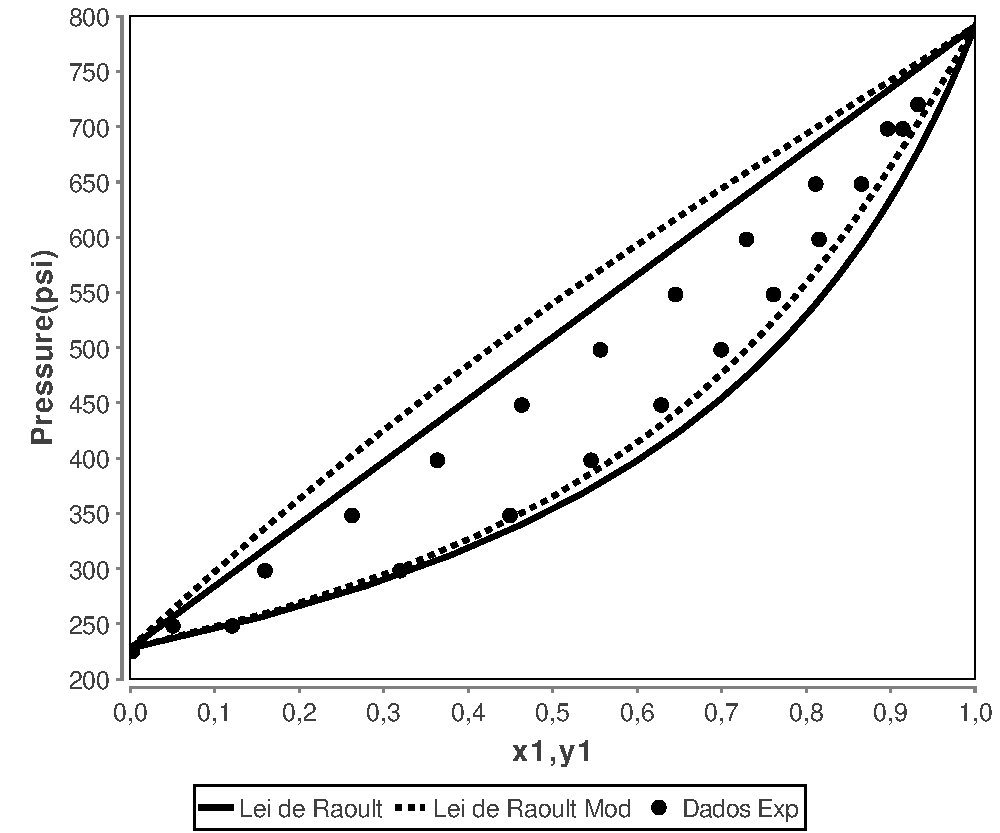
\includegraphics[width=0.8\textwidth]{img/VLE-Ethane(1)Propylene(2)-x1y1&Pressure-Raoult-RaoultMod.pdf}}
\caption{Diagrama de equilíbrio $P-xy$ da mistura de etano (1) e
propeno (2) calculados com as Leis de Raoul e Raoult Modificada utilizando
modelo de atividade UNIFAC(Do)}
\label{fig:raoult01}
\end{figure}

A \autoref{fig:raoult02} mostra um comparativo dos valores de fração molar da
fase gasosa e da fase líquida para o etano utilizando as leis de Raoult e Raoult
Modificado via UNIFAC (Do). Observa-se que as curvas ficaram distantes dos
pontos experimentais exceto para pressões mais baixas.

\begin{figure}[htb]
\centering
{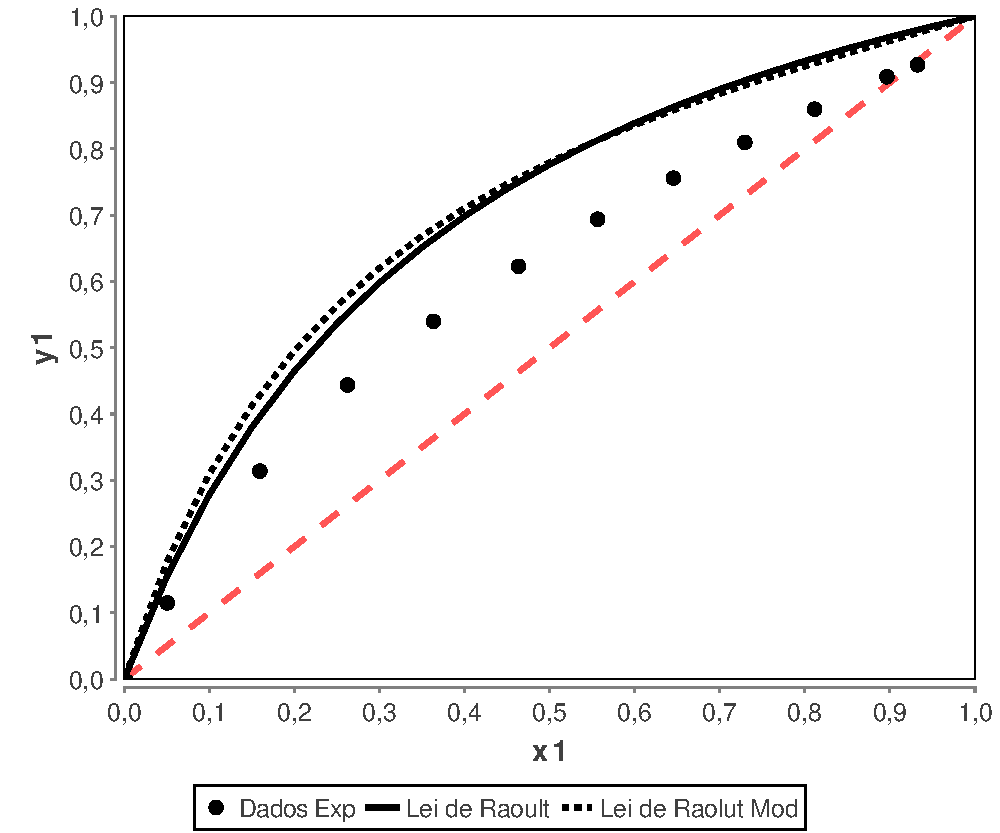
\includegraphics[width=0.8\textwidth]{img/VLE-Ethane(1)Propylene(2)-x1&y1-Raoult-RaoultMod.pdf}}
\caption{Diagrama de equilíbrio $y-x$ da mistura de etano (1) e
propeno (2) calculados com as Leis de Raoul e Raoult Modificada utilizando
modelo de atividade UNIFAC(Do)}
\label{fig:raoult02}
\end{figure} 


\subsection{Método $\phi-\phi$} 

As Figuras \ref{fig:phi01} e \ref{fig:phi02} apresentam a predição do método
$\phi-\phi$ utilizando Peng-Robinson como equação de estado para a mistura
etano e propeno. Apesar das mesmas não evidenciarem os valores
extremos, tais mostram que tal método obteve uma melhor predição dos valores
experimentais quando comparada àquelas mostradas nas Figuras
\ref{fig:raoult01} e \ref{fig:raoult02}.

\begin{figure}
\centering
{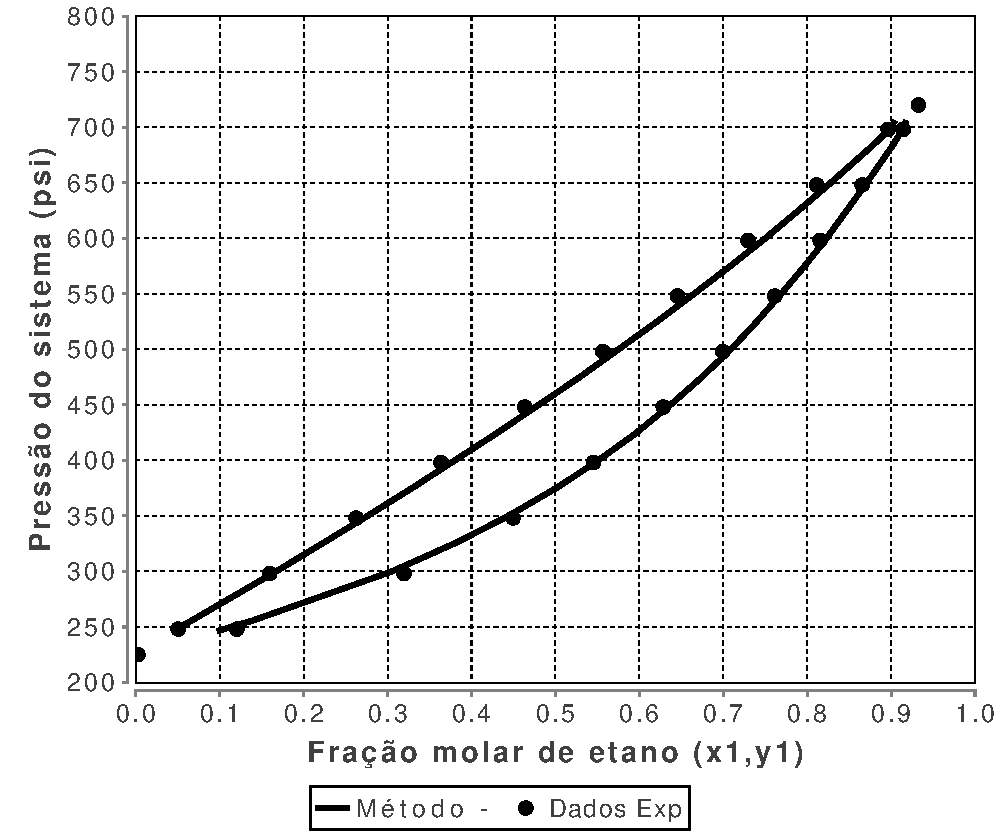
\includegraphics[width=0.8\textwidth]{img/VLE-Ethane(1)Propylene(2)-x1y1&Pressure-PengRobinson.pdf}}
\caption{Diagrama de equilíbrio $P-xy$ da mistura de de etano (1) e
prepeno (2) calculados com as EoSs PR}
\label{fig:phi01}
\end{figure}

\begin{figure}
\centering
{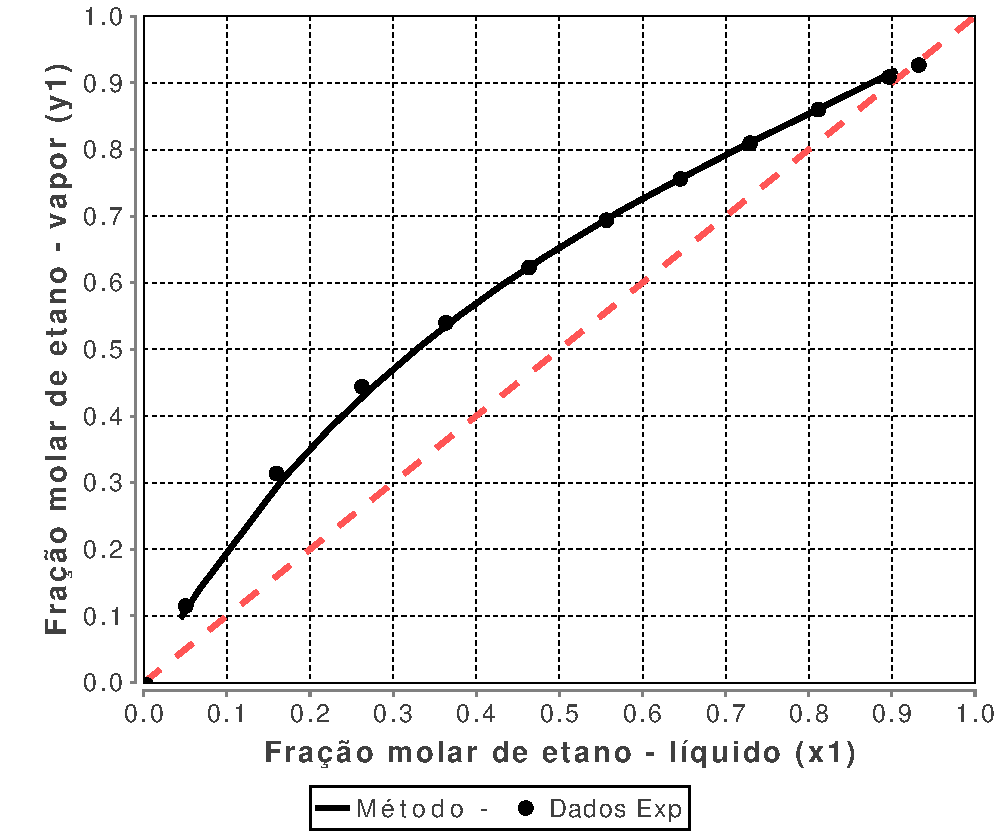
\includegraphics[width=0.8\textwidth]{img/VLE-Ethane(1)Propylene(2)-x1&y1-PengRobinson.pdf}}
\caption{Diagrama de equilíbrio $y-x$ da mistura de de etano (1) e
prepeno (2) calculados com as EoSs PR}
\label{fig:phi02}
\end{figure}
\clearpage

\section{Conclusões}

Este trabalho visou o estudo da predição e construção de diagramas de equílibrio
líquido-vapor (mistura etano e propeno) utilizando diferentes modelos de
cálculo. Foram utilizadas as Leis de Raoult e Raoult Modificada (com UNIFAC(Do)
para cálculo do coeficiente de atividade) e o modelo $\phi-\phi$ utilizando Peng-Robinson como equação de
estado e os valores preditos foram comparadas qualitativamente a dados
experimenais.

A partir dos resultados apresentados, conclui-se que o modelo $\phi-\phi$
preveu melhor os valores experimentais, visto que esse método considera ambas as
fases sendo não ideais. Tanto a lei de Raoult, como a lei de Raoult modificada,
apresentaram resultados menos satisfatórios para tais cálculos, sendo que a
primeira considera ambas as fases ideais e a segunda faz a consideração de
líquido não ideal. 

Os valores obtidos para o líquido, foram melhores aproximados pela lei de
Raoult Modificada. Já os do vapor, foram aproximados melhor através da Lei de Raoult.
Contudo, nenhum desses modelos foi capaz de prever o
comportamento supercrítico do etano.


  
%\section{Introdução Teórica}

\subsection{Equações de Estados}

\begin{equation}\label{eq:001}
P = \frac{RT}{v - b} - \frac{\alpha(T)}{(v + \epsilon b)(v + \sigma b)}
\end{equation}

$\alpha = \displaystyle\frac{\Psi\alpha(T_r)R^2T_c^2}{P_c}$

$b = \displaystyle\Omega\frac{RT_c}{P_c}$

$T_r = \displaystyle\frac{T}{T_c}$

$P_r = \displaystyle\frac{P}{P_c}$

\subsubsection{Peng-Robinson}




\section{Conclusões}





%\section{Objetivos}
O presente trabalho tem por objetivo construir uma curva de EFV (do
ingês, \emph{equilibrium flash vaporization}) para um petróleo qualquer. A
composição do óleo será determinada a partir de valores de TBP (do ingês,
\emph{true boiling point} - ponto de ebulição verdadeiro) obtidos de
informações fornecidadas pelo site da TOTSA.

Para isso, inicialmente será realizada uma breve contextualização de alguns
tópicos, tais como análises de TBP e EFV, bem como algumas regras de mistura
que serão usadas no trabalho.

\section{Introdução teórica}

\subsection{TBP}
A curva de TBP (\emph{true boiling point}) ou PEV (ponto de ebulição verdadeiro)
é um gráfico que contem os valores dos pontos de ebulição  dos componentes quase puros q
ue estão contidos em um petróleo bruto ou em alguma de suas frações. Antigamente, 
essa curva era construída em laboratório utilizando equipamentos complexos de 
destilação em batelada com cem ou mais estágios de equilíbrio e alta razão de 
refluxo. Hoje em dia, esse mesmo gráfico é feito por meio de espectroscopia de massa, 
muito mais rápida e com precisão mais elevada \cite{Jones2006}.

\subsection{EFV}


A curva EFV (\emph{equilibrium flash vaporization}) fornece a informação da
temperatura que um dado volume de destilado será vaporizado. Esse vapor
destilado está sempre em equilíbrio com a fase líquida e os ensaios de EFV são
sempre conduzidos em pressão atmosférica. De acordo com \citeonline{Eckert2008},
esse ensaio é raramente realizado, pois é muito trabalhoso. Em uma série de
experimentos, são medidas as temperaturas de equilíbrio para diferentes valores especificados de 
 fração de líquidos. Esse tipo de ensaio também é usado para projetar processos
 onde ocorre equilíbrio líquido-vapor como, por exemplo, refervedores, condesadores
  parciais, etc).
  
\subsection{Equação de Estados: Peng-Robinson}

 A equação de \citeonline{Peng1976}, apresentada na
 \autoref{eq:PReq}, faz o uso do fator acêntrico de Pitzer ($w$). Com esse 
 parâmetro, espera-se que esse modelo seja melhor aplicado para diferentes classes
 de moléculas \cite{Koretsky2013}.
      
\begin{equation}\label{eq:PReq}
P = \frac{RT}{v - b} - \frac{\alpha T(r)}{v(v+b)+b(v-b)}
\end{equation} 

O valor de $\alpha T(r)$ é descrito na \autoref{eq:alfa}:
 \begin{equation}\label{eq:alfa}
\alpha T(r) = [1 +
 \kappa(1-\sqrt{T_r})]^2
\end{equation} 
onde $\kappa = (0,37464+1,54226w-0,26992w^2)$. 
 O fator acêntrico de Pitzer caracateriza o quão ``não-esférica'' é a molécula,
 assim, pode ser atribuída para uma classe de substâncias com
 características semelhantes. A \autoref{eq:w} apresenta a definição desse fator
 acêntrico:
 
  \begin{equation}\label{eq:w}
w \equiv -1 - log_{10}\left [ P^{sat} \left ( T_r = 0,7 \right )/P_c \right ]
\end{equation} 
onde $ P^{sat} \left ( T_r = 0,7 \right )$ é a pressão de saturação de dada
substância em uma termperatura reduzida igual a 0,70.

\subsection{Regras de Mistura}

\citeonline{Koretsky2013} afirma que a abordagem mais prática no uso de equações de estado
é utilizar regras de mistura que se baseiam nos dados dos componentes puros e 
aplicam tais para os tipos de interações presentes na mistura em questão. A 
\autoref{eq:aij} apresenta a formulação para o termo relacionado à força de
atração entre duas moléculas diferentes em uma mistura.

\begin{equation}\label{eq:aij}
a_{mix} = \sum_i\sum_jy_iy_ja_{ij}
\end{equation}
onde $y$ são as frações molares dos componentes $i$ e $j$ e $a_{ij}$ é a
atração entre as molecúlas dos mesmos componentes $i$ e $j$. O termo de atração
da \autoref{eq:aij} segue as premissas apresentadas a seguir, nas Equações
\ref{eq:aij2}, \ref{eq:aij3} e \ref{eq:aij4}. 

\begin{equation}\label{eq:aij2}
a_{ij} = a_{ji}
\end{equation}

\begin{equation}\label{eq:aij3}
a_{ij} = \sqrt{a_ia_j}(1 - k_{ij})
\end{equation}

\begin{equation}\label{eq:aij4}
a_{i} = a_{ii}
\end{equation}

A \autoref{eq:bmix} apresenta a expressão para o termo relacionado ao volume
excluído quando ocorre a mistura.

\begin{equation}\label{eq:bmix}
b_{mix} = \sum_iy_ib_i
\end{equation}

\subsubsection{van der Waals (vdW)}
\citeonline{Kwak1986} mostra que, para uma mistura binária cuaj energia potencial
intermolecular expressa na \autoref{eq:uij}, as regras de mistura derivadas são 
as Equações \ref{eq:sigmacubo} e \ref{eq:esigmacubo}.

\begin{equation}\label{eq:uij}
u_{ij}(r) = \epsilon_{ij}f(r/\sigma_{ij})
\end{equation}

\begin{equation}\label{eq:sigmacubo}
\sigma^3 = \sum_i^n\sum_j^nx_ix_j\sigma_{ij}^3
\end{equation}

\begin{equation}\label{eq:esigmacubo}
\varepsilon\sigma^3 = \sum_i^n\sum_j^nx_ix_j\varepsilon_{ij}\sigma_{ij}^3
\end{equation}
onde $\varepsilon_{ij}$ é o parâmetro de interação energética entre as moléculas
$i$ e $j$, e $\sigma_{ij}$ é a distância de interação intermolecular entre duas
moléculas. Os coeficientes $a$ e $b$ da equação de estado de van der Waals são
proporcionais aos valores de $\varepsilon$ e $\sigma$.

Sabendo que $\sigma_{ij}$, para $i \neq j$, a interação entre diâmetro
distintos, para moléculas esféricas, é mostrado na \autoref{eq:sigmaij}

\begin{equation}\label{eq:sigmaij}
\sigma_{ij} = \frac{\sigma_{ii} + \sigma_{jj}}{2}
\end{equation}

Tal leva a seguinte expressão de $b_{ij}$ para moléculas esféricas, conforme
\autoref{eq:bij}

\begin{equation}\label{eq:bij}
b_{ij} = \left ( \frac{b_{ii}^{1/3} + b_{jj}^{1/3}}{2} \right )^3
\end{equation}

E, para moléculas não esféricas, a relação é descrita na \autoref{eq:bij2}

\begin{equation}\label{eq:bij2}
b_{ij} = (1 - l_{ij})\left [ b_{ii}^{1/3} + b_{jj}^{1/3} \right ]^3
\end{equation}

\subsubsection{Regra de Mistura vdW para EoS PR}

A equação de Peng-Robinson (\autoref{eq:PReq}) pode ser reescrita como mostrado
na \autoref{eq:PRnew}

\begin{equation}\label{eq:PRnew}
Z = \frac{\nu}{\nu - b} - \frac{(a/RT) + d - 2 \sqrt{ad/RT}}{(\nu + b) +
(b/\nu)(\nu - b)}
\end{equation}
onde: $a = a(T_c)(1 + \kappa)^2$ e $d =
\displaystyle\frac{a(T_c)\kappa^2}{RT_c}$.

Assim, a equação de estado de Peng-Robinson apresenta 3 termos
independentes: $a$, $b$ e $d$. Deste modo, seguindo o modelo antes mostrado para
regras de mistura de van der Waals, tem-se:

\begin{equation}\label{eq:PRnew1}
a = \displaystyle\sum_i^n\sum_j^nx_ix_ja_{ij}
\end{equation}
\begin{equation}\label{eq:PRnew2}
b = \displaystyle\sum_i^n\sum_j^nx_ix_jb_{ij}
\end{equation}
\begin{equation}\label{eq:PRnew3}
d = \displaystyle\sum_i^n\sum_j^nx_ix_jd_{ij}
\end{equation}
onde: 
\begin{equation}\label{eq:PRnew4}
a_{ij} = (1 - k_{ij})\sqrt{a_{ii}a_{jj}}
\end{equation}
\begin{equation}\label{eq:PRnew5}
b_{ij} = (1 - l_{ij})\left [ \frac{b_{ii}^{1/3} + b_{jj}^{1/3}}{2} \right]^3
\end{equation}
\begin{equation}\label{eq:PRnew6}
d_{ij} = (1 -m_{ij})\left [ \frac{d_{ii}^{1/3} + d_{jj}^{1/3}}{2} \right]^3
\end{equation}
\subsubsection{SCMR}
Conforme é apresentado por \citeonline{Staudt2012}, esta regra de
mistura apresenta volume de excesso negligenciável e a fração $ u =
\frac{V}{b} $ é constante. A \autoref{eq:gphi1} apresenta a expressão para
energia de Gibbs em excesso e a \autoref{eq:lnphi} para o coeficiente de
fugacidade para mistura.

\begin{equation}\label{eq:gphi1}
\frac{G_\phi^E}{RT} = ln\phi - \sum_ix_iln\phi_i
\end{equation}

\begin{equation}\label{eq:lnphi}
ln\phi = (Z - 1) - ln(Z - \beta) + qI
\end{equation}

Utilizando a definição de volume em excesso ($V^E$) e abrindo o termo $ln(Z -
\beta)$, obtem-se a \autoref{eq:gphi2}:

\begin{equation}\label{eq:gphi2}
\frac{G_\phi^E}{RT} = \frac{PV^E}{RT} + \sum_ix_iln\left ( \frac{V_i - b_i}{V -
b} \right ) + qI - \sum_ix_iq_iI_i
\end{equation}

Assumindo que o volume em excesso é negligenciável, obtem-se a
\autoref{eq:gphi3}:

\begin{equation}\label{eq:gphi3}
\frac{G_\phi^E}{RT} = \sum_ix_iln\left ( \frac{V_i - b_i}{V^{Id} -
b} \right ) + qI^{Id} - \sum_ix_iq_iI_i
\end{equation}
onde $b$ é calculado via \autoref{eq:bmix}, o volume das substâncias puras
$V_i$, bem como $I^{Id}$ e $I_i$, devem ser calculados utilizando a raiz do tipo
líquido do sistema puro nas temperaturas e pressões do sistema. Para baixas pressões, pode-se igualar os
 modelos de Gibbs em excesso para a fugacidade e o coeficiente de atividade
 ($G_\phi^E$ = $G_\gamma^E$).

\subsubsection{PSRK}

No trabalho de \citeonline{Chen2002}, é mostrado como é obtido o parâmetro $a$.
A expressão para tal é ilustrada na \autoref{eq:abrt}.


\begin{equation}\label{eq:abrt}
\frac{a}{bRT} = \sum x_i\frac{a_{ii}}{b_iRT}+\frac{1}{A}\left (
\frac{g_0^E}{RT}+\sum x_iln\frac{b}{b_i} \right )
\end{equation}
onde $A$ foi setado como -0,64663. \citeonline{Fischer1996} afirmam
que PSRK gera bons resultados para as propriedades termodinâmicas, especialmente para 
equilíbrios líquido-vapor em altas pressões.

\subsection{Modelo de Atividade: Scatchard-Hildebrand}
Segundo \citeonline {Brignole2013}, a teoria de soluções regulares de
Scatchard-Hildebrand provém do modelo de Flory-Huggins considerando que a entropia da mistura corresponde ao valor 
de uma mistura ideal. Além disso, ela leva em consideração a existência do 
calor da mistura que ocorre devido às interações energéticas moleculares. 
Uma vez que todas as combinações em uma mistura binária sejam levadas em 
conta, a expressão para o coeficiente de atividade do componente 1 é
apresentada na \autoref{eq:lngamma1}:

\begin{equation}\label{eq:lngamma1}
ln\gamma_1 = \frac{\nu_1\varphi_2^2(\delta_1-\delta_2)^2}{RT}
\end{equation}
onde $\gamma_1$é o coeficiente de atividade e $\nu_1$ é o volume molar para o
componente 1 e $\varphi_2$ é a fração volumétrica do componente 2. Os parâmetros
de solubilidade dos componentes puros ($\delta_1$ e $\delta_2$) podem ser
obtidos a partir da energia interna de vaporização de cada componente puro $i$
($\Delta u_i^v$), como um líquido saturado na temperatura do sistema
(\autoref{eq:deltai}):

\begin{equation}\label{eq:deltai}
\delta_i = \left ( \frac{\Delta u_i^V}{\nu_i^L} \right )^{\frac{1}{2}}
\end{equation}

O termo entre parânteses da \autoref{eq:deltai} é denominado de densidade de energia
coesiva e o parâmetro de solubilidade para misturas multicomponentes é mostrada
na \autoref{eq:delta}:

\begin{equation}\label{eq:delta}
\delta = \sum_i\sum_j\phi_i\phi_j\delta_{ij}^2
\end{equation}

onde

\begin{equation}\label{eq:deltaij}
\delta_{ij}^2 = \delta_1\delta_j
\end{equation}

Assim, substituindo a \autoref{eq:deltaij} na \autoref{eq:delta}, pode-se obter
uma nova expressão $\delta$, como é mostrado na \autoref{eq:delta2}.

\begin{equation}\label{eq:delta2}
\delta = \sum_i\phi_i\delta_i
\end{equation}


\section{Metodologia}

\subsection{Dados experimentais}

Para a realização do trabaho, foram utilizados dados de análise de um
petróleo do poço CLOV localizado na Angola. Essa informação foi
coletada no site da \emph{Total Oil Trading S.A.} (\citeauthor{TOTSA2016}). O
principal fator para a escolha desse poço foi que a última análise do óleo foi
realizada recentemente, em janeiro de 2016. Os resultados das análises
físico-químicas do pretróleo, bem como os dados de Pronto de Ebulição Verdadeiro
(PEV ou TBP) estão mostrados nas Tabelas \ref{tab:dados} e \ref{tab:tbp}.

\begin{table}[htb]
\renewcommand{\arraystretch}{1.3}
\caption{Característica do petróleo extraído do poço CLOV - Angola}
\footnotesize 
\center
\begin{tabular}{llc}
\toprule
 {Data da análise}						&						&	{25/01/20016}	\\
 {Densidade a 15$^\circ$C (kg/m$^3$)}	&						&	{858,9}			\\
 {$^\circ$API}							&						&	{33,2}			\\
 {Bbl/mt}								&						&	{7,336}			\\
 {Acidez (mg KOH/g)}					&						&	{0,54}			\\
 {Enxofre (massa\%)}					&						&	{0,249}			\\
 {Sulfeto de Hidrogênio (mg/kg)}		&						&	{1}				\\
 {Enxofre de mercaptanos (mg/kg)}		&						&	{3}				\\
 {Viscosidade (cSt)} 					&		{10 $^\circ$C}	&	{19,3}			\\
 { }				 					&		{50 $^\circ$C}	&	{5,4}			\\
 {Ponto de Fluidez ($^\circ$C)}			&						&	{-6}			\\
 {Nitrogênio total (massa\%)}			&						&	{0,142}			\\
 {Cera (massa\%)}						&						&	{-}				\\
 {Temp. aparente de cera  ($^\circ$C)}	&						&	{-}				\\
 {RVP a 37,8 $^\circ$C (kPa)}			&						&	{26}			\\
 {Umidade (vol\%)}						&						&	{-}				\\
 {NaCl (mg/kg)}							&						&	{-}				\\
 {Níquel (mg/kg)}						&						&	{7,7}			\\
 {Vanádio (mg/kg)}						&						&	{1,9}			\\
 {Ferro (mg/kg)}						&						&	{-}				\\
 {Mercúrio ($\mu$g/kg)}					&						&	{-}				\\
 {Leves (vol\%)}						&	{Etano}				&	{0,06}			\\
 										&	{Propano}			&	{0,57}			\\
 										&	\emph{iso}-Butano	&	{0,33}			\\
 										&	\emph{n}-Butano		&	{0,94}			\\
\bottomrule
\multicolumn{3}{c}{Fonte: \citeonline{TOTSA2016}}
\end{tabular}
\label{tab:dados}
\end{table}
\clearpage

\begin{table}[htb]
\renewcommand{\arraystretch}{1.3}
\caption{Dados de Ponto de Ebulição Verdadeiro (PEV ou TBP)
para o poço CLOV - Angola}
\sisetup{table-format=2.2,round-mode=places,round-precision=2}
\footnotesize
\center
\begin{tabular}{S[table-format=3.0,round-mode=places,round-precision=0]SS|S[table-format=3.0,round-mode=places,round-precision=0]SS}
\toprule
   {T} & {\%. vap.} & {\% vap.}&{T} &
   {\% vap.} & {\% vap.}\\
   {($^\circ$C)} & {(massa)} & {(vol.)}&{($^\circ$C)} &
   {(massa)} & {(vol.)}\\
\midrule 
80  &4.88  &6.60&  340 & 49.61 &53.57\\
90  &5.83  &7.73&  360 & 53.30 &57.18\\
100 &7.01  &9.10&  380 & 56.86 &60.64\\
120 &10.02 &12.54& 400 & 60.31 &63.96\\
140 &13.62 &16.56& 420 & 63.66 &67.16\\
160 &17.05 &20.31& 440 & 66.91 &70.25\\
180 &19.98 &23.47& 460 & 70.06 &73.22\\
200 &22.86 &26.52& 480 & 73.09 &76.05\\
220 &26.08 &29.90& 500 & 75.99 &78.75\\
240 &29.72 &33.65& 520 & 78.73 &81.28\\
260 &33.64 &37.67& 540 & 81.30 &83.64\\
280 &37.71 &41.78& 560 & 83.68 &85.81\\
300 &41.78 &45.85& 580 & 85.87 &87.80\\
320 &45.76 &49.80&     &       &     \\
\bottomrule
\multicolumn{6}{c}{Fonte: \citeonline{TOTSA2016}}
\end{tabular}
\label{tab:tbp}
\end{table}

\subsection{Procedimento de Cálculo}
Para a obtenção da curva EFV, foram utilizados os dados experimentais
de TBP e fez-se o uso do simulador de processo $iiSE$. O modelo termodiâmico
utilizado foi o de Peng-Robinson com três diferentes regras de mistura: van der
Waals (vdW), PSRK e SCMR. Para as duas últmas, é necessário o uso de um modelo
de Gibbs em excesso ($g^E$), portanto utilizou-se para ambas o modelo de
Scatchard-Hildebrand.

Para a configuração do petróleo no $iiSE$, foram inseridos os valores dos
percentuais volumétricos dos quatro leves contidos nos resultados da análise experimental e
foi feito um corte em 30 pseudos. Para a avaliação da composição do líquido e do
vapor em função do percentual vaporizado, utilizou-se apenas as frações dos
leves e de 6 pseudos com massas molares distintas, os quais foram escolhidos
aleatoriamente.

\clearpage 

\section{Resultados} 

Realizou-se a simulação da curva de EFV no \emph{software} $iiSE$, para todas as
regras de misturas, variando-se a temperatura de 0,0 $^\circ$C até 600,0
$^\circ$C, com passo de $\Delta$T unitário. Deste modo, foram obtidos 600 pontos
para cada simulação, com o intuito de, além de construir a curva EFV, poder
fazer uma comparação entre cada teste.

Primeiramente, buscou-se conhecer qual foi a temperatura onde iniciou-se a
vaporização do componente mais leve e o instante onde ocorre a vaporização do
mais pesado. Contudo, observa-se que, nas condições utilizadas no presente
trabalho, o simulador apresentou dificuldade na predição dos valores quando a
vaporização aproximou-se de 90,5{\%}. Deste modo, considerou-se, então, que a
temperatura final a ser comparada seria exatamente a anterior àquela que o
simulador não foi capaz de predizer corretamente. A \autoref{tab:result1}
apresenta os valores de temperatura (inicial e final da vaporização), bem como o
passo de $\Delta$T.

\begin{table}[htb]
\renewcommand{\arraystretch}{1.3}
\caption{Temperaturas, iniciais e finais, e passos de T para cada regra de
mistura na simulação EFV para o óleo CLOV - Angola}
\sisetup{table-format=2.2,round-mode=places,round-precision=2}
\footnotesize
\center 
\begin{tabular}{lccc}   
\toprule
   &{Temperatura Inicial}&{Temperatura Final}&\multirow{2}{*}{$\Delta$T} \\
  &{da Fração Vaporizada ($^\circ$C)}&{da Fração Vaporizada
   ($^\circ$C)} & \\
\midrule 
{EFV: PR+SCMR}	&	73	&	472		&	1 \\
{EFV: PR+VDW}	&	75	&	468		&	1 \\
{EFV: PR+PSRK}	&	51	&	469		&	1 \\
\bottomrule
%\multicolumn{4}{c}{Fonte: \citeonline{TOTSA2016}}
\end{tabular}
\label{tab:result1}
\end{table}

A \autoref{fig:efv} apresenta os resultados simulados para as curvas EFV
utilizando a equação de estado Peng-Robinson com as diferentes regras de
mistura. Além disso, está graficada a curva TBP do óleo, cujos dados foram
obtidos do laudo de análise do mesmo.
\clearpage

\begin{figure}[htb]
\centering
{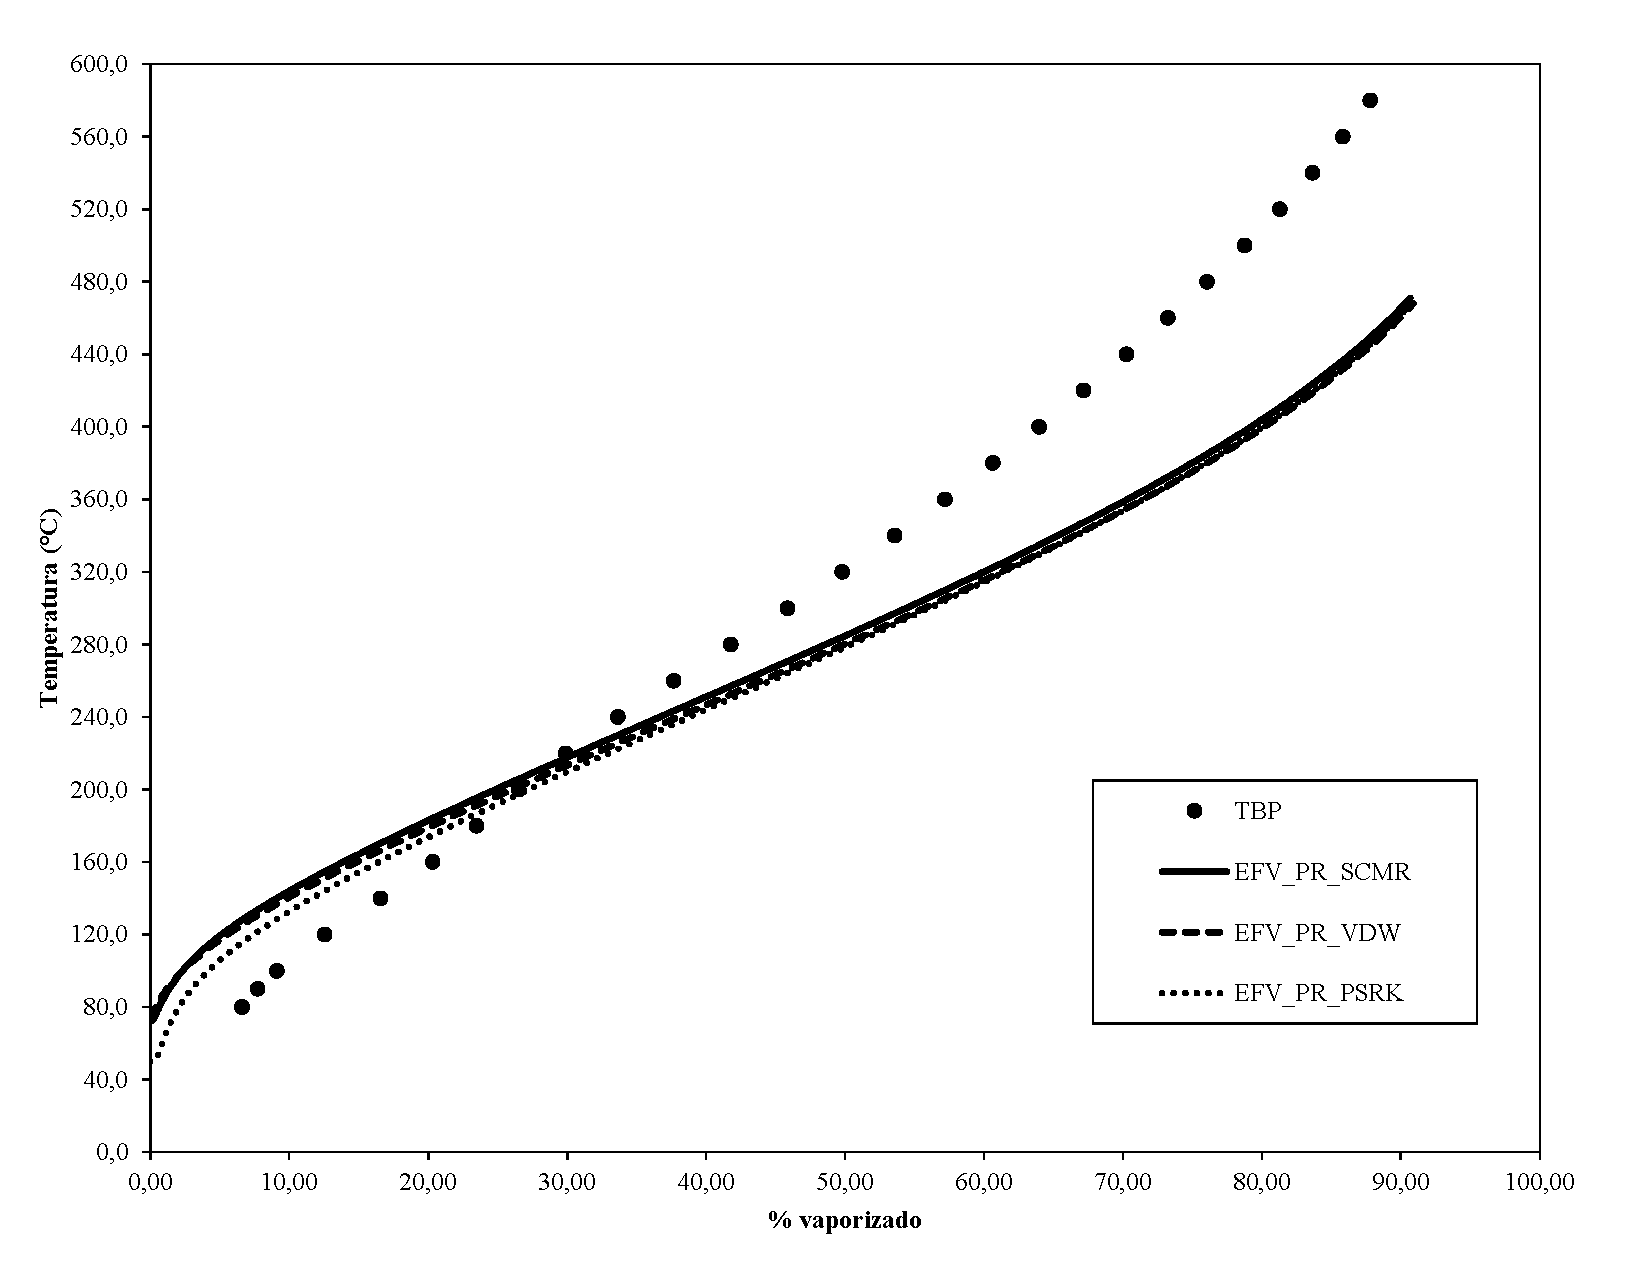
\includegraphics[width=1.0\textwidth]{img/trab3.pdf}} 
\caption{Curva de TBP e EFV para o petróleo do poço CLOV - Angola}
\label{fig:efv}
\end{figure} 


Ao analisar a \autoref{fig:efv}, nota-se que as curvas EFV com as regras de
mistura SCRM e vdW apresentaram comportamentos semelhantes. Contudo, ao
utilizar-se PSRK (\emph{Predictive Soave-Redlich-Kwong}), observa-se um desvio
considerável nos valores iniciais, quando comparado às outras duas. Este fato pode ser explicado devido à não utilização
do ``pacote fechado'' desta regra de mistura, uma vez que para o modelo de Gibbs
em excesso foi utilizado Scatchard-Hildebrand ao invés do UNIFAC(PSRK). Além
disso, a equação de estado a ser utilizado devia ser SRK
(\emph{Soave-Redlich-Kwong}) e não Peng-Robinson.

Os dados apresentados na \autoref{tab:result2} referem-se ao comparativo, passo
a passo, do percentual vaporizado entre as regras de mistura. O objetivo é saber
se, em algum momento dentro da faixa de temperatura avaliada, há uma
diferença significativa da percentagem vaporizada, quando as regras de mistura
são analisadas (duas a duas). Nesse intuito, comparou-se apenas os modelos de
mistura quando ambos detinham percentual vaporizada diferente de zero e/ou menor
que 90,5 {\%}.

\clearpage
\begin{table}[htb]
\renewcommand{\arraystretch}{1.3}
\caption{Comparativo entre os desvios no percentual vaporizado de cada regra de
mistura}
\sisetup{table-format=2.2,round-mode=places,round-precision=2}
\footnotesize
\center 
\begin{tabular}{lcc}   
\toprule
  {Regras de Mist.} &{Máx. Diferença}&{Faixa de Máx.} \\
   {Comparadas}&{do \% Vaporizada*}&{diferença de T ($^\circ$C)} \\
\midrule 
{SCMR - vdW}	&	1.34	&	{256 - 257}	 \\
{SCMR - PSRK}	&	2.55	&	{151 - 159}	 \\
{vdW - PSRK}	&	1.88	&	{112 - 118}	 \\
\bottomrule
\multicolumn{3}{l}{*Diferenças apresentadas em módulo}
\end{tabular}
\label{tab:result2}
\end{table}

A partir da \autoref{tab:result2}, observa-que a faixa de temperatura para o
terceiro comparativo (vdW - PSRK) ocorre em uma faixa de temperatura menor que
as demais. Portanto, a mesma acontece quando a percentual vaporizada detém
valores pequenos (faixas entre 4,13 a 6,0 {\%}), ou seja, trata-se de uma
diferença significativa (desvio de 31{\%}). A diferença (relativa) do percentual
vaporizado para o primeiro e segundo comparativo apresentado na tabela foram,
respectivamente, 3,0 e 18,0 {\%}.

\clearpage


\begin{figure}[htb]
\centering
{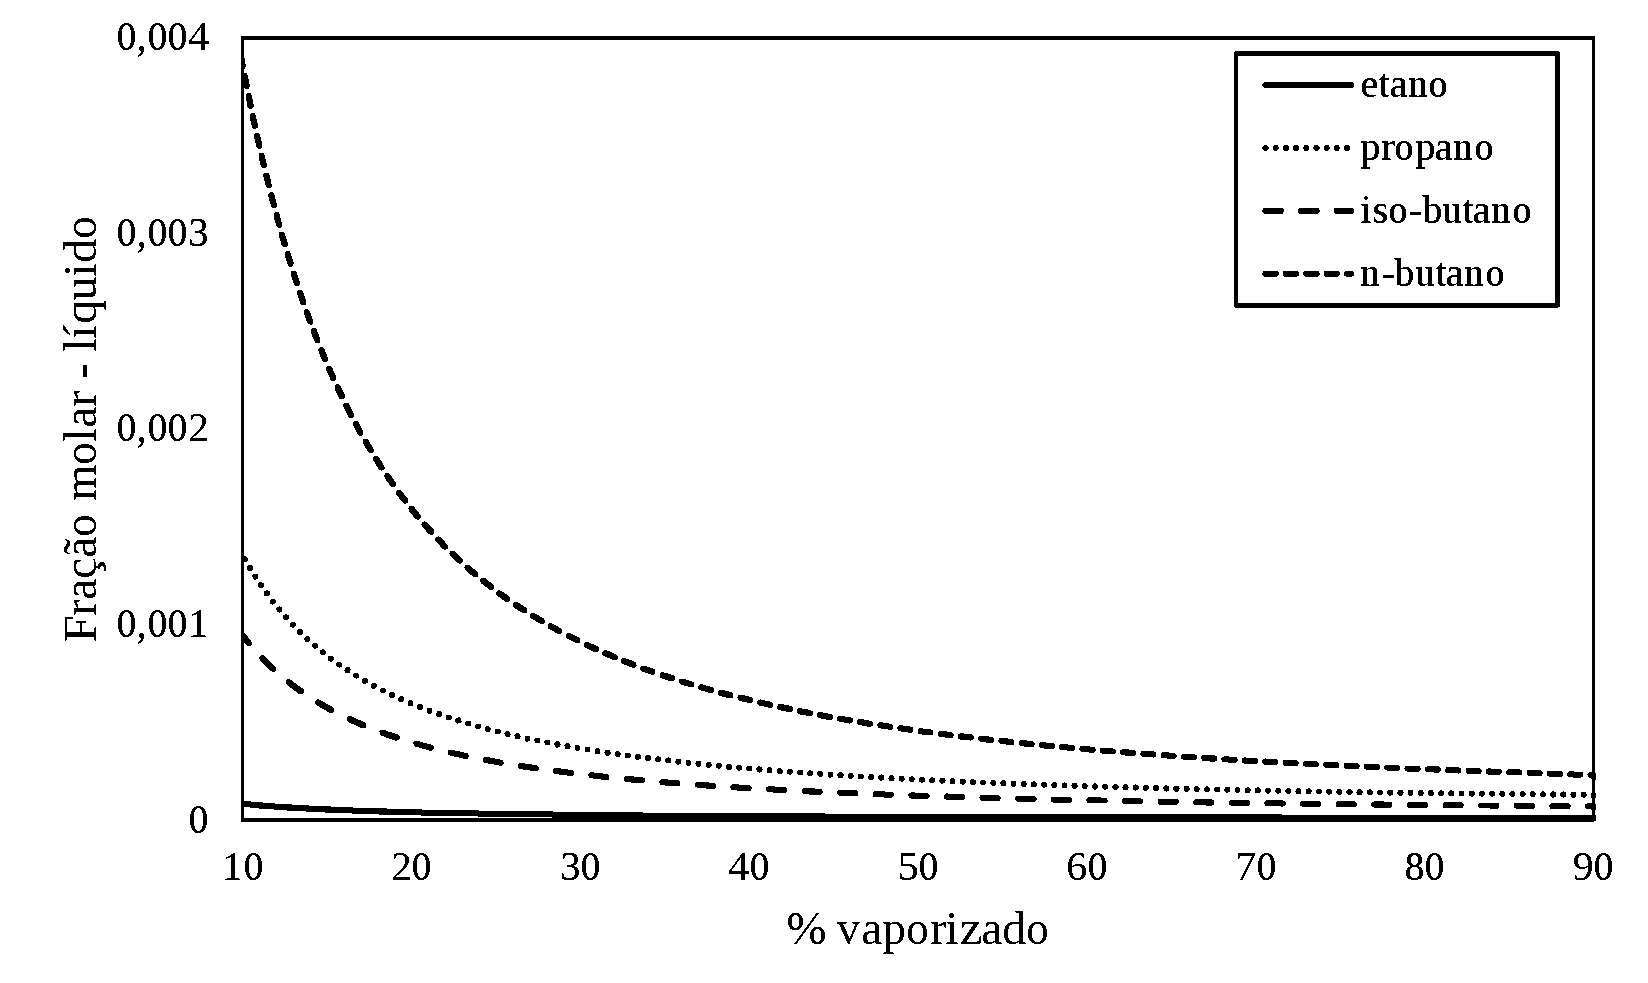
\includegraphics[width=1.0\textwidth]{img/trab3liq.pdf}} 
\caption{Composição dos leves no produto de fundo em função do
percentual vaporizado}
\label{fig:liq}
\end{figure}

\begin{figure}[htb]
\centering
{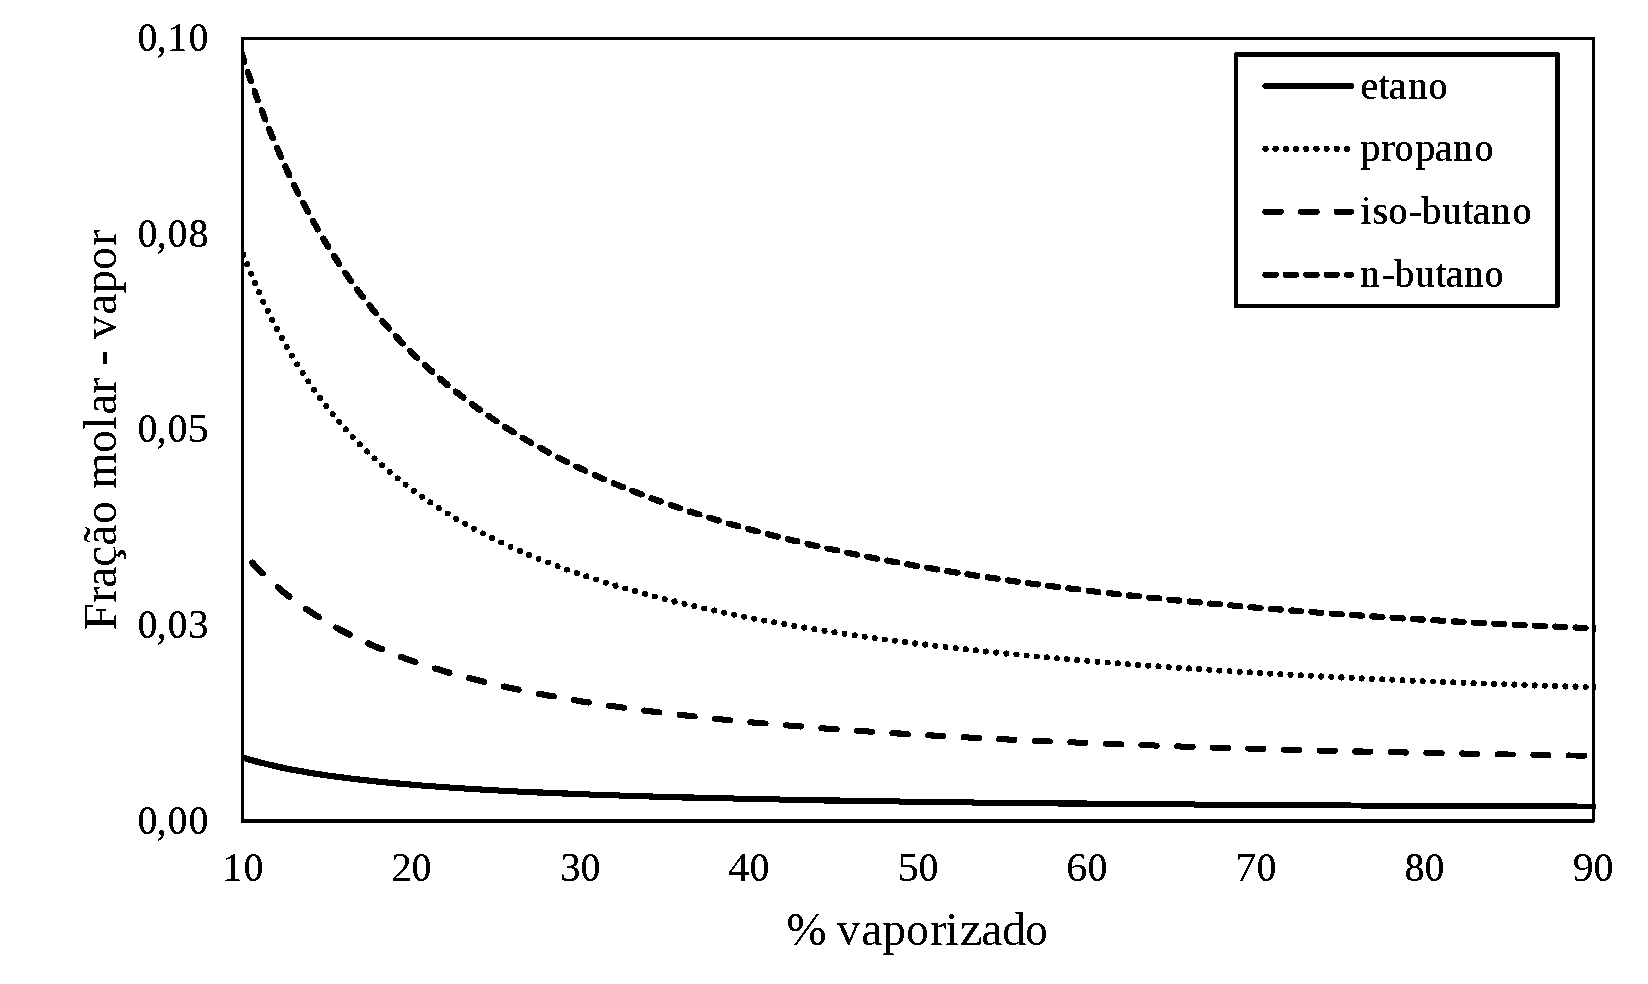
\includegraphics[width=1.0\textwidth]{img/trab3vap.pdf}} 
\caption{Composição dos leves no produto de topo em função do percentual
vaporizado}
\label{fig:vap}
\end{figure}

\begin{figure}[htb] 
\centering
{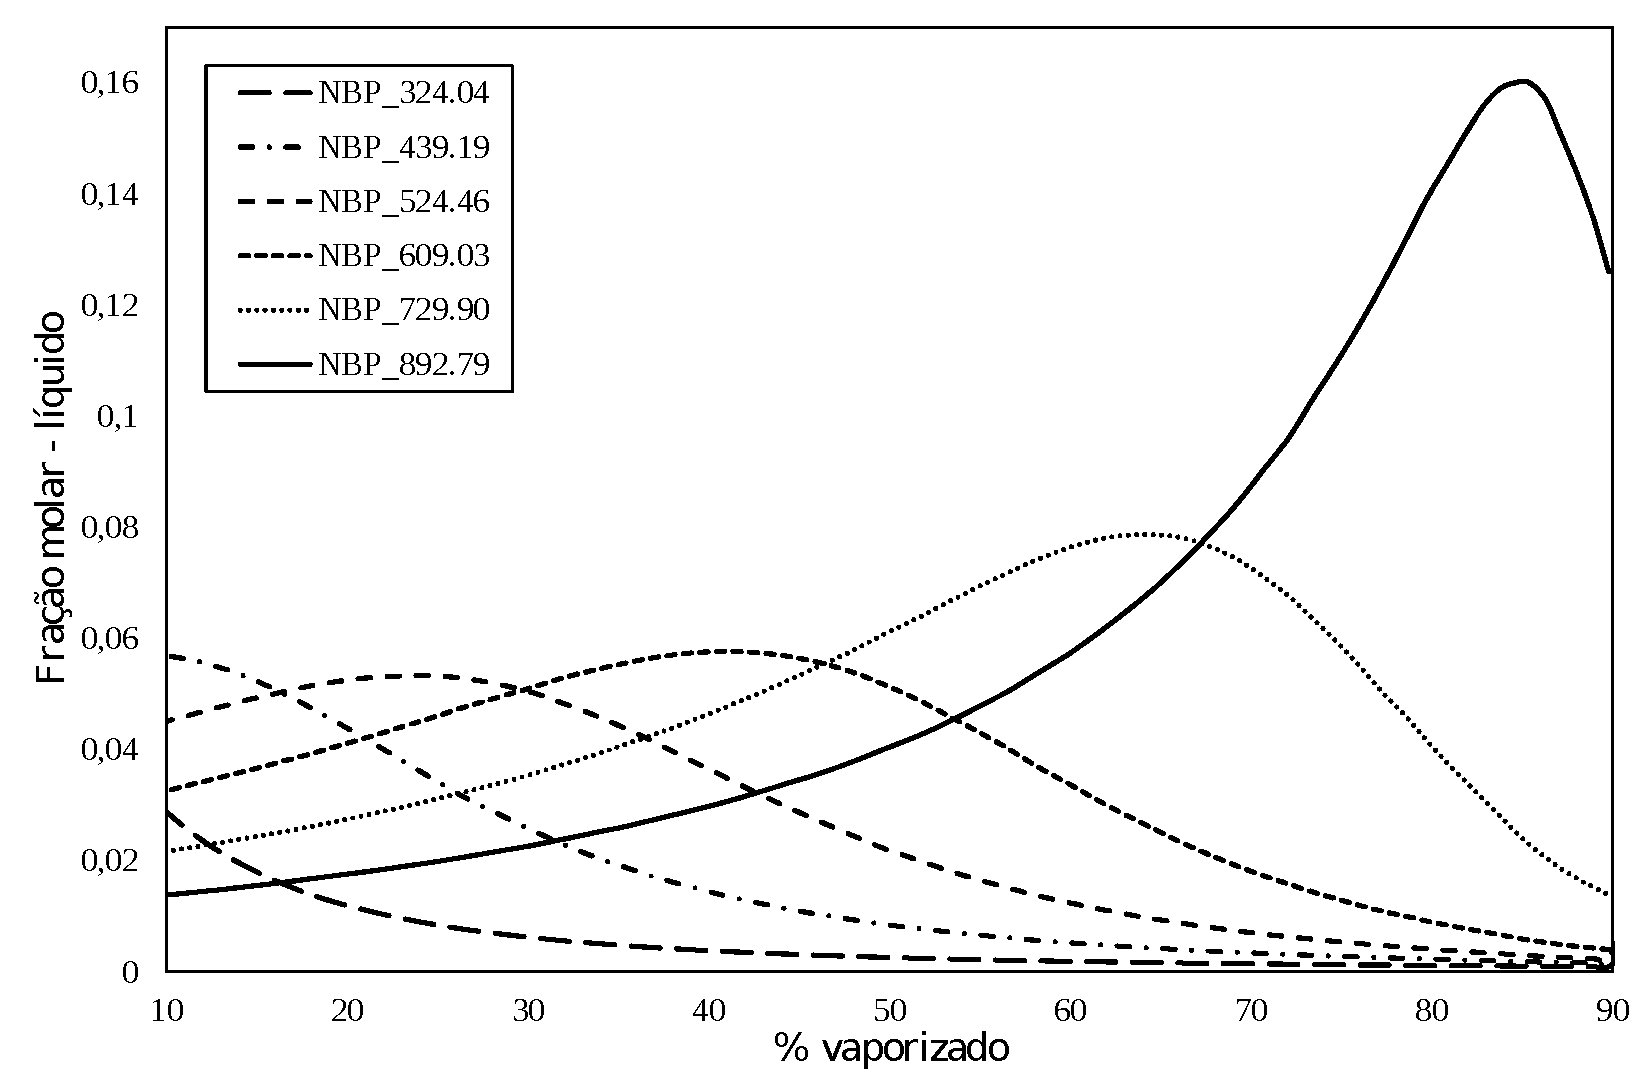
\includegraphics[width=1.0\textwidth]{img/trab3liqall.pdf}} 
\caption{Composição de alguns pseudos no produto de fundo em função do
percentual vaporizado}
\label{fig:liqall}
\end{figure}

\begin{figure}[htb]
\centering
{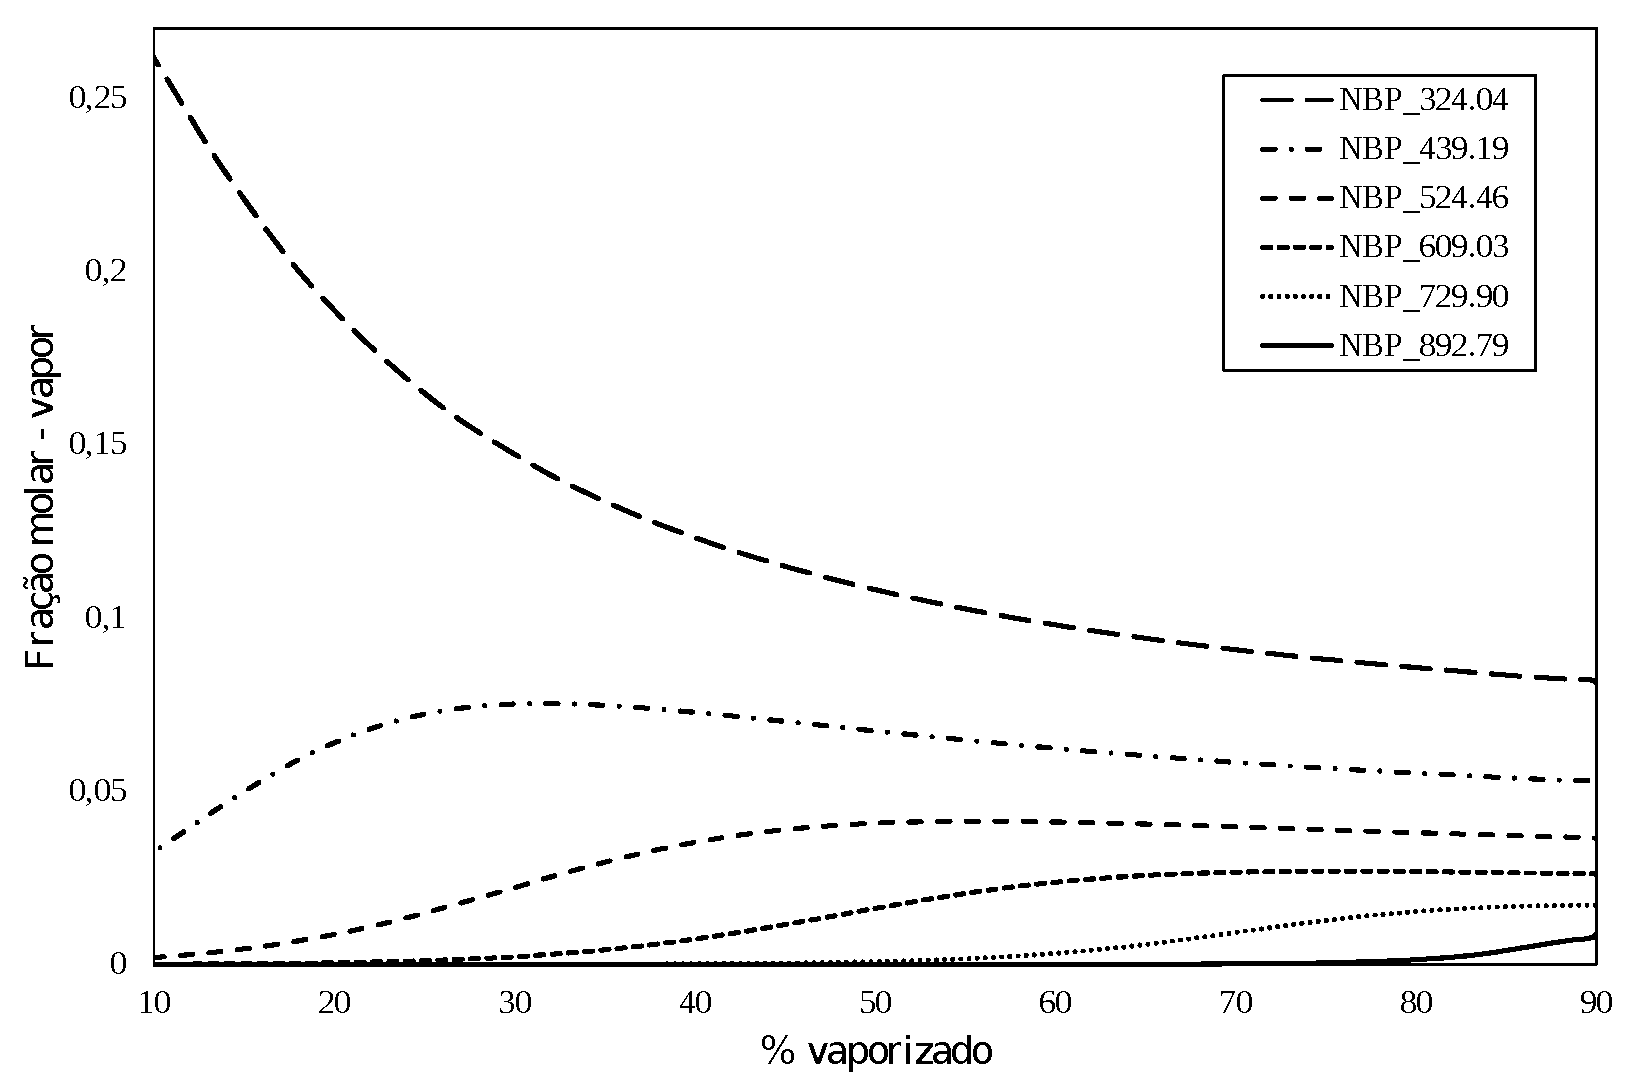
\includegraphics[width=1.0\textwidth]{img/trab3vapall.pdf}} 
\caption{Composição de alguns pseudos no produto de topo em função do
percentual vaporizado}
\label{fig:vapall}
\end{figure}

\clearpage
\section{Conclusões}  


%\section{Objetivos}
O presente trabalho tem por objetivo construir um diagrama de equilíbrio
líquido-vapor (ELV) para uma mistura de um polímero (poliisobutileno - PIB) com
um solvente (benzeno). Para isso, será apresentada uma breve discussão dos
modelos e metodologia de cálculo, assim como a teoria aplicada.

\section{Introdução Teórica}


A teoria de \citeonline{Flory1951} e \citeonline{Huggins1942} considera a
energia livre de Gibbs da mistura do polímero puro com o solvente
($\Delta g_{mis}$) em termos de duas contribuições: entalpia de mistura 
($\Delta h_{mis}$) e entropia de mistura ($\Delta s_{mis}$), conforme é
apresentado a seguir:

\begin{equation}\label{eq:gemist}
\Delta g_{mis} = \Delta h_{mis} - T\Delta s_{mis}
\end{equation}
onde $T$ é a temperatura absoluta.

A entropia de mistura é determinada pelas frações volumétricas do solvente
($\phi_1$) e do polímero ($\phi_2$), enquanto a entalpia é determinada pelo
parâmetro adimensional de interação $\chi$, o qual normalmente é referido como parâmetro de interação de
Flory-Huggins, conforme é apresentado nas equações abaixo: 

\begin{equation}\label{eq:entalexc}
\Delta h_{mis} = \chi RT\left( x_1 + mx_2 \right)\phi_1\phi_2
\end{equation}

\begin{equation}\label{eq:entroexc}
\Delta s_{mis} = -R\left( x_1\ln\phi_1 + x_2\ln\phi_2 \right)
\end{equation}

De acordo com \citeonline{Koretsky2013}, a energia de Gibbs em
excesso ($g^E$) é expressa através da diferença entre $\Delta g_{mis}$ e sua
condição ideal, como mostrado abaixo:

\begin{equation}\label{eq:geexc1}
g^E = \Delta g_{mis} - \Delta g_{mis}^{ideal}
\end{equation}
onde:

\begin{equation}
\Delta g_{mis}^{ideal} = RT\sum_ix_i\ln x_i
\end{equation}

Substituindo na \autoref{eq:geexc1}, obtem-se:

\begin{equation}
g^E = \Delta g_{mis} - RT\sum_ix_i\ln x_i
\end{equation}

Através da definição de $\Delta g_{mis}$ e considerando um sistema binário,
tem-se:

\begin{equation}\label{eq:geexc2}
g^E = \Delta h^{mist} - T\Delta s^{mist} - RT\left( x_1\ln x_1 + x_2\ln x_2
\right)
\end{equation}

Substituindo as Equações \ref{eq:entalexc} e \ref{eq:entroexc} na
\autoref{eq:geexc2} e fazendo-se as devidas simplificações, obtem-se uma
expressão para a energia de Gibbs em excesso em função das frações molares
($x_i$) e volumétricas ($\phi_i$), como é apresentado abaixo:

\begin{equation}\label{eq:geRT}
\frac{g^E}{RT} = \chi\left(x_1 + mx_2\right)\phi_1\phi_2 +
\left[x_1\ln\frac{\phi_1}{x_1} + x_2\ln\frac{\phi_2}{x_2}\right]
\end{equation}
onde $x_1$ e $x_2$ são as frações molares do solvente e do polímero,
respectivamente; $\phi_1$ e $\phi_2$ são, respectivamente, as frações
volumétricas do solvente e polímero, as quais são obtidas através das
seguintes equações:

\begin{equation}\label{eq:fracvap}
\phi_1 = \frac{n_1}{n_1 + mn_2}
\end{equation}

\begin{equation}
\phi_2 = \frac{mn_2}{n_1 + mn_2} = 1 - \phi_1
\end{equation}
onde $m$ é o número de repitições da unidade de monômero contida na cadeia
polimérica e pode ser obtida através da razão entre massa molar do polímero
($M_{wp}$) pela do monômero ($M_{wm}$), como é apresentado a seguir:

\begin{equation}
m = \frac{M_{wp}}{M_{wm}}
\end{equation}

 Aplicando-se a definição de uma
propriedade parcial molar para a \autoref{eq:geRT}, ou seja, realizando-se a
diferenciação com relação ao número de mols do solvente, obtem-se
a seguinte expressão para o coeficiente de atividade para tal
componente da mistura ($\gamma_1$):


\begin{equation}\label{eq:gamma1}
\ln\gamma_1 = \ln\frac{\phi_1}{x_1} + \phi_2\left( 1 - \frac{1}{m} \right) +
\chi\phi_2^2
\end{equation}

De uma maneira análoga ao que foi feito para a obtenção da \autoref{eq:gamma1},
chega-se na seguinte expressão do coeficiente de atividade para o polímero
($\gamma_2$):

\begin{equation}
\ln\gamma_2 = \ln\frac{\phi_2}{x_2} - \phi_1\left( m - 1 \right) +
m\chi\phi_1^2
\end{equation}

Conforme é apresentado por \citeonline{Tadros2013}, o parâmetro de interação de
Flory-Huggins ($\chi$) fornece a medida da interação das cadeias poliméricas com as moléculas de solvente e, também, as interações
polímero-polímero. 

Quando $\chi$ assume valor igual a $1/2$, o polímero se comporta
como uma mistura ideal com o solvente e, nessa condição, é denotado por Flory
como ponto $\theta$. Desse modo, o polímero não sofre nenhum tipo de repulsão ou
atração. Para valores de $\chi$ inferiores a $1/2$, a mistura
se comporta como não ideal, apresentando desvios positivos (repulsão). 
Em contrapartida, para $\chi$ superior a $1/2$, ocorrem desvios negativos
(atração). Nessas condições, pode haver a precipitação do polímero.

Conforme é apresentado por \citeonline{Lindvig2002}, a relação entre o parâmetro
de interação de Flory-Huggins e o parâmetro de solubilidade é apresentada
através da seguinte expressão:

\begin{equation}
\chi = \frac{v_1}{RT}\left( \delta_1 - \delta_2 \right)^2
\end{equation}

Os parâmetros
de solubilidade dos componentes puros ($\delta_1$ e $\delta_2$), conforme
\citeonline{Kwak1986}, podem ser obtidos a partir da energia interna de
vaporização de cada componente puro $i$ ($\Delta u_i^v$), como um líquido saturado na temperatura do sistema
(\autoref{eq:deltai}):

\begin{equation}\label{eq:deltai}
\delta_i = \left ( \frac{\Delta u_i^V}{\nu_i^L} \right )^{\frac{1}{2}}
\end{equation}

O termo entre parânteses da \autoref{eq:deltai} é denominado de densidade de energia
coesiva e o parâmetro de solubilidade para misturas multicomponentes é mostrada
na \autoref{eq:delta}:

\begin{equation}\label{eq:delta}
\delta = \sum_i\sum_j\phi_i\phi_j\delta_{ij}^2
\end{equation}
onde

\begin{equation}\label{eq:deltaij}
\delta_{ij}^2 = \delta_i\delta_j
\end{equation}



\section{Metodologia}

Para a realização do estudo do equilíbrio líquido-vapor da mistura
polímero - solvente contendo benzeno e poliisobutileno (PIB) utilizaram-se 
os dados experimentais (retirados do material fornecido em aula) apresentados na
\autoref{tab:dexp2}. As propriedades, necessárias para os cálculos, das duas
substâncias envolvidas no estudo estão mostradas na \autoref{tab:dexp1}.

\begin{table}[htb]
\renewcommand{\arraystretch}{1.3}
\centering
\caption{Dados experimentais de ELV da mistura polímero-solvente benzeno(1) /
PIB(2) a 312,75 K.}
\begin{tabular}{S[table-format=2.2,round-mode=places,round-precision=2]
S[table-format=1.4,round-mode=places,round-precision=4]}
\toprule
{$w_1$ (\%)}	&	{P (bar)}	\\
\midrule

4,37	&	0,0715	\\
6,33	&	0,0971	\\
9,45	&	0,1236	\\
15,16	&	0,1681	\\
18,42	&	0,1818	\\
25,37	&	0,2095	\\
29,71	&	0,2182	\\
32,12	&	0,2207	\\
37,30	&	0,2267	\\
\bottomrule
\end{tabular}
\label{tab:dexp2} 
\end{table} 

\begin{table}[htb]
\renewcommand{\arraystretch}{1.3}
\caption{Propriedades dos componentes da mistura polímero-solvente benzeno(1) /
PIB(2)}
\sisetup{table-format=2.2,round-mode=places,round-precision=2}
\footnotesize
\center
\begin{tabular}{lrlr}
\toprule
\multicolumn{2}{c}{Benzeno (1)}	&	\multicolumn{2}{c}{PIB (2)}		\\
\cmidrule(lr{.5em}){1-2} \cmidrule(lr{.5em}){3-4}
{$M_{w1}\rm{ (g/mol)}$} 	&	{$78$}	&	{$M_{wp}\rm{ (g/mol)}$}	&	{$40000$}	\\
{$v_1\rm{ (cm^3/mol)}$}	&	{$88,26$}	&	{$M_{wm} \rm{ (g/mol)}$}	&	{$104$}	\\
{$P_1^{sat}\rm{ (bar)}$}	&	{$0,2392$}	&	{$v_m \rm{ (cm^3/mol)}$}	&	{$131,9$}	\\

\bottomrule
\multicolumn{4}{c}{Obs.: Dados retirados do material fornecido em aula}
\end{tabular}
\label{tab:dexp1}
\end{table}

Apenas para nível de comparação, a \autoref{tab:prop1} mostra alguns valores
experimentais de $\chi$ para a mistura benzeno/PIB para diferentes composições e
faixas de temperaturas.

\clearpage

\begin{table}[htb]
\centering
\renewcommand{\arraystretch}{1.3}
\caption{Valores experimentais de $\chi$ em função da temperatura e da fração
volumétrica do polímero ($\phi_2$) encontrados na literatura}
\begin{tabular}{lcc}
\toprule
{Temperatura ($^\circ$C)} & {Fração Volumétrica ($\phi_2$)} & {$\chi$}		\\
\midrule
{$	10			$}	&	{$	0,4$	a	$0,8$}	&	{$	0,670$	a	$0,920$	}	\\
{$	25			$}	&	{$	0,0$	a	$1,0$}	&	{$	0,498$	a	$1,060$	}	\\
{$	25			$}	&	{$	1,0$	 		}	&	{$	0,880$	a	$0,610$	}	\\
{$	27$	a	$65	$}	&	{$	0,6$	a $1,0$	}	&	{$	0,730$	a	$1,070$	}	\\
{$	30			$}	&	{$	0,0$			}	&	{$	0,495$				}	\\
{$	40			$}	&	{$	0,6$	a $0,8$	}	&	{$	0,700$	a	$0,800$	}	\\
{$	50			$}	&	{$	0,0$	a $0,2$	}	&	{$	0,485$	a	$0,583$	}	\\
{$	100			$}	&	{$	1,0$			}	&	{$	0,700$				}	\\
{$	37$	a	$200$}	&	{$	1,0$			}	&	{$	1,180$	a	$0,700$	}	\\

\bottomrule
\multicolumn{3}{c}{Fonte:\citeonline{Orwoll2007}}
\end{tabular}
\label{tab:prop1}
\end{table}

Para os cálculos de equilíbrio, utilizou-se o modelo da Lei de Raoult
Modificada, considerando a fase vapor como sendo um gás ideal. O coeficiente de
atividade foi calculado através do modelo de Flrory-Huggins, explanado na seção
anterior.

\begin{equation}
\hat{f_1}^l = \hat{f_1}^v
\end{equation}

\begin{equation}
\gamma_1x_1P_1^{sat} = Py_1
\end{equation}

Como o solvente apresenta-se na forma pura na fase vapor, ou seja, sua fração
molar ($y_1$) é igual a 1,0, tem-se:

\begin{equation}
\gamma_1x_1P_1^{sat} = P
\end{equation}

Como os dados de composição foram apresentados em base mássica, foi necessário
convertê-los em base molar para fazer-se o uso do modelo. A seguir está mostrada
a relação entre as frações mássicas e molares:

\begin{equation}
x_1
=\frac{\displaystyle
\frac{w_1}{M_{w1}}}{\displaystyle\frac{w_1}{M_{w1}}+\frac{w_2}{M_{wp}}}
\end{equation}

A partir disso, é possível reescrever a \autoref{eq:fracvap} em função das
frações mássicas e volumes molares, como é apresentado a seguir:

\begin{equation}
\phi_1 =
\frac{\displaystyle\frac{w_1}{M_{w1}}v_1}{\displaystyle\frac{w_1}{M_{w1}}v_1+\displaystyle\frac{w_2}{M_{wp}}mv_m}
\end{equation}

Os códigos de programação foram implementados em
liguagem $Java$ utilizando o ambiente do Eclipse Mars 2 Release (4.5.2)


\section{Resultados}

\subsection{Sensibilidade do modelo aos valores de $\chi$ }
Nessa seção buscou-se ententer o comportamento do modelo frente a diferentes
valroes de $\chi$. A \autoref{tab:allsets} apresenta as configurações utilizadas
para cada cálculo e utilizou-se $0,50$ como valor inicial de $\chi$ (mistura
ideal) até o valor máximo de $1,50$, com passo de $0,10$.

\begin{table}[htb]
\centering
\renewcommand{\arraystretch}{1.3}
\caption{Valores dos erros médios (absoluto e relativo) para diferentes valores
do parâmetro de interação polímero-solvente ($\chi$)}
\begin{tabular}{S[table-format=3.0,round-mode=places,round-precision=0]
S[table-format=2.0,round-mode=places,round-precision=0]
S[table-format=1.2,round-mode=places,round-precision=2]
S[table-format=1.2,round-mode=places,round-precision=2]}
\toprule
{Valores de}& {Quantidade de} & \multirow{2}{*}{$\chi_{min}$} &
\multirow{2}{*}{$\chi_{max}$}\\
{$w_1$ gerados}& {$\chi$ testados} & &\\
\midrule
100&11&0.5&1.5\\
\bottomrule
\end{tabular}
\label{tab:allsets}
\end{table}

Foram testados, posteriormente, valores de $\chi$ inferiores a $0,50$ e
superiores a $1,50$, porém os resultados apresentaram-se com desvios maiores
com relação aqueles avaliados. Conforme o apresentado na
\autoref{tab:prop1}, praticamente todos os valores de $\chi$ para a mistura em
questão apresentam-se dentro da faixa avaliada.

A \autoref{tab:allresult} apresenta os valores médios dos erros absoluto e
relativo para todos os valores de $\chi$ avaliados. Observa-se que os menores erros
médios ocorrem quando $\chi$ é igual a $1,00$. A \autoref{fig:trab4ki} mostra os
comportamentos do modelo na predição do equilíbrio, frente aos diferentes
valores de $\chi$, comparados com os dados experimentais. Os valores pontuais de
erro absoluto e relativo encontram-se no Apêndice A.

\clearpage

\begin{table}
\centering
\renewcommand{\arraystretch}{1.3}
\caption{Valores dos erros médios (absoluto e relativo) para diferentes valores
do parâmetro de interação polímero-solvente ($\chi$)}
\begin{tabular}{cS[table-format=1.4,round-mode=places,round-precision=4]S[table-format=2.2,round-mode=places,round-precision=2]}
\toprule
& {Erro Médio} & {Erro Médio} 	\\
& {Absoluto} & {Relativo (\%)}	 \\
\midrule 
{$\chi = 0,50$} & 0.0431 & 29.06 \\
{$\chi = 0,60$} & 0.0352 & 24.26 \\
{$\chi = 0,70$} & 0.0268 & 19.11 \\
{$\chi = 0,80$} & 0.0179 & 13.58 \\
{$\chi = 0,90$} & 0.0105 & 8.61  \\
{$\chi = 1,00$} & 0.0093 & 6.38  \\
{$\chi = 1,10$} & 0.0147 & 7.81  \\
{$\chi = 1,20$} & 0.0244 & 12.88 \\
{$\chi = 1,30$} & 0.0368 & 20.77 \\
{$\chi = 1,40$} & 0.0501 & 29.24 \\
{$\chi = 1,50$} & 0.0643 & 38.34 \\
\bottomrule
\end{tabular}
\label{tab:allresult}
\end{table}

\begin{figure}
\centering
{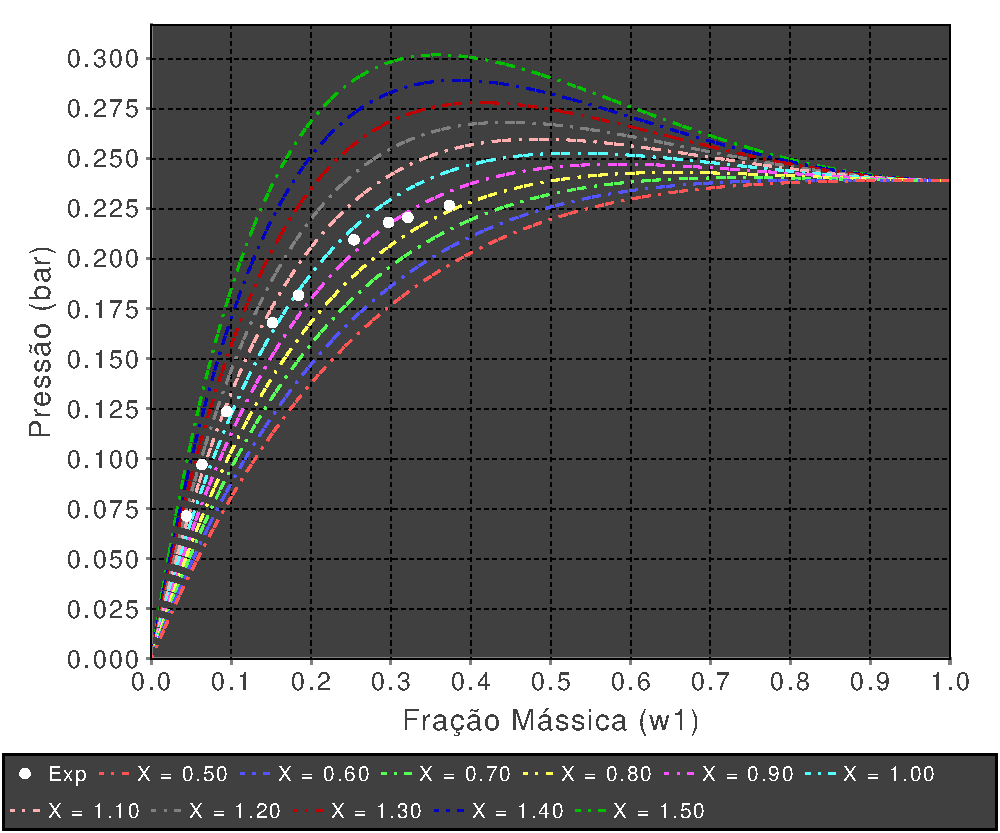
\includegraphics[width=0.8\textwidth]{img/Trab4Ki.pdf}} 
\caption{Curvas $P-w_1$ para diferentes valores de $\chi$}
\label{fig:trab4ki}
\end{figure}

\clearpage

\subsection{Otimização}
Otimização de processos pode ser matematicamente descrita como uma busca por um
máximo ou mínimo de uma função objetivo. Assim, neste trabalho, a função objetivo escolhida 
foi o somatório do diferencial da pressão calculada a partir dos parâmetros
$\chi$ com a pressão experimental. Entretanto, mediante à possibilidade de
avaliação de tais erros ser feita por mais de uma forma, escolheu-se investigar duas 
alternativas: erro médio absoluto e erro médio relativo.

A metodologia de otimização utilizada foi a \emph{simplex Nelder-Mead}, uma vez
que esta possui uma convergência veloz para uma função objetivo simples. A inicialização 
foi realizada, em ambos os casos, considerando a \autoref{tab:OptT1}  como
configuração inicial.

\begin{table}[htb]
\centering
\renewcommand{\arraystretch}{1.3}
\caption{Configuração inicial das otimizações}
\begin{tabular}{S[table-format=1.2,round-mode=places,round-precision=2]
S[table-format=1.2,round-mode=places,round-precision=2]
S[table-format=4.0,round-mode=places,round-precision=0]
c}
\toprule
{$\chi_0$}& {$\chi_1$} & {N$^\circ$ máx. de iterações} & {Tolerância} 	\\
\midrule
0,50&0,60&8000&{$10^{-10}$}\\
\bottomrule
\end{tabular}
\label{tab:OptT1}
\end{table}

\subsubsection{Otimização - Erro Absoluto}
A função objetivo utilizada para o erro absoluto é mostrada na
\autoref{eq:fobjabs}. A minimização é feita alterando o valor de $\chi$ e a
função objetivo é um somatório, para todos os pontos avaliados (NP), da
diferença, em módulo, da pressão experimental ($P^{exp}$) e da pressão calculada via o modelo
($P^{calc}$).

\begin{equation}\label{eq:fobjabs}
min_\chi f_{obj} = \sum_i^{NP}\frac{1}{NP}\left| P_i^{exp} -
P_i^{calc} \right|
\end{equation}

A \autoref{fig:trab4abs} mostra o comportamento do modelo para diferentes
valores de $\chi$, bem como a curva otimizada para o erro absoluto. Observa-se
que a curva otimizada passa exatamente sobre o quinto ponto experimental (ponto
médio). Já a \autoref{tab:Opt2T1} apresenta os valores alcançados pela
otimização e o valor de $\chi$ ótimo ($\chi_{opt}$). Os valores relativos a
cada ponto experimental estão presente no Apêndice B.

\begin{figure}[htb]
\centering
{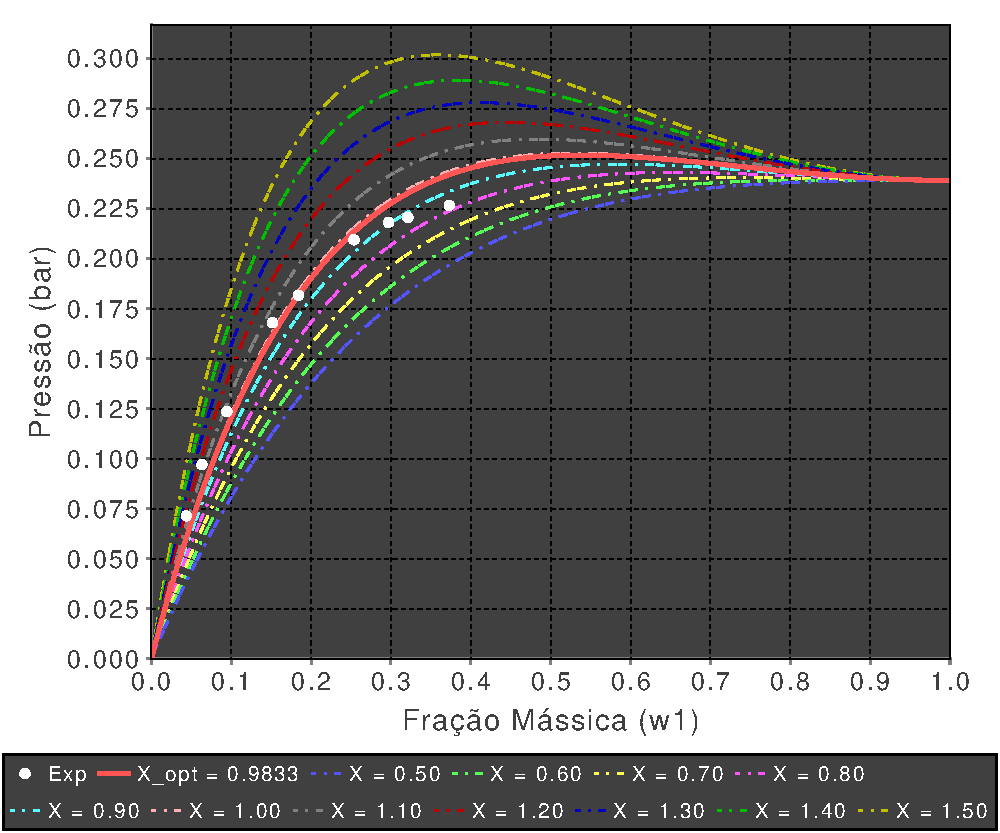
\includegraphics[width=0.8\textwidth]{img/Trab4Abs.pdf}} 
\caption{Curvas $P-w_1$ para diferentes valores de $\chi$ com valor otimizado
(minimizando a diferença dos erros absolutos)}
\label{fig:trab4abs}
\end{figure}



\begin{table}[htb]
\centering
\renewcommand{\arraystretch}{1.1}
\caption{Resposta da otimização com o erro médio absoluto como função
objetivo}
\begin{tabular}{S[table-format=1.4,round-mode=places,round-precision=4]
S[table-format=1.4,round-mode=places,round-precision=4]
S[table-format=1.4,round-mode=places,round-precision=4]
S[table-format=2.0,round-mode=places,round-precision=0]
S[table-format=1.4,round-mode=places,round-precision=4]}
\toprule
\multirow{2}{*}{$\chi_{opt}$}& {Erro Abs.} & {Erro Rel.} & {N$^\circ$
iterações} & {Valor da}\\
& {Médio} & {Médio ($\%)$} & {realizadas} & {$f_{obj}$}\\
\midrule
0.9833&0.0089&6.4287&38&0.0089\\
\bottomrule
\end{tabular}
\label{tab:Opt2T1}
\end{table}

\subsubsection{Otimização - Erro Relativo}
A função objetivo utilizada para o erro relativo é mostrada na
\autoref{eq:fobjrel}. A minimização é feita alterando o valor de $\chi$ e a
função é um somatório, para todos os pontos avaliados (NP), da diferença, em módulo, da pressão 
experimental ($P^{exp}$) e da pressão calculada via o modelo ($P^{calc}$),
divindido tal pela pressão experimental.

\begin{equation}\label{eq:fobjrel}
min_\chi f_{obj} = \sum_i^{NP}\frac{1}{NP}\left| \frac{P_i^{exp} -
P_i^{calc}}{P_i^{exp}} \right|
\end{equation}


A \autoref{fig:trab4rel} mostra o comportamento da função para diferentes
valores de $\chi$, bem como a curva otimizada para o erro relativo. Observa-se
que, desta vez, a curva otimizada passa exatamente sobre o quarto ponto
experimental. Já a \autoref{tab:Opt3T1} apresenta os valores alcançados pela
otimização e o valor de $\chi$ ótimo ($\chi_{opt}$). Os valores relativos a cada
ponto experimental estão presente no Apêndice B.


\begin{figure}[htb]
\centering
{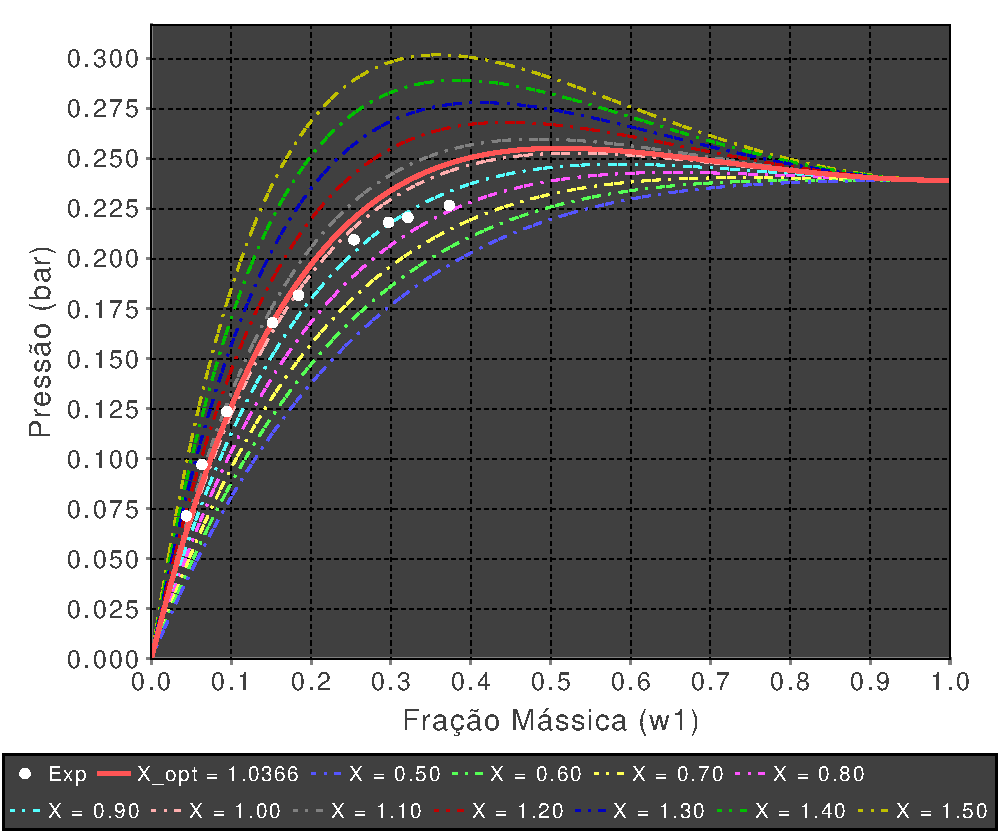
\includegraphics[width=0.8\textwidth]{img/Trab4Rel.pdf}} 
\caption{Curvas $P-w_1$ para diferentes valores de $\chi$ com valor otimizado
(minimizando a diferença  dos erros relativos)}
\label{fig:trab4rel}
\end{figure}

\begin{table}[htb]
\centering
\renewcommand{\arraystretch}{1.1}
\caption{Resposta da otimização com o erro médio relativo como função
objetivo}
\begin{tabular}{S[table-format=1.4,round-mode=places,round-precision=4]
S[table-format=1.4,round-mode=places,round-precision=4]
S[table-format=1.4,round-mode=places,round-precision=4]
S[table-format=2.0,round-mode=places,round-precision=0]
S[table-format=1.4,round-mode=places,round-precision=4]}
\toprule
\multirow{2}{*}{$\chi_{opt}$}& {Erro Abs.} & {Erro Rel.} & {N$^\circ$
iterações} & {Valor da}\\
& {Médio} & {Médio ($\%)$} & {realizadas} & {$f_{obj}$}\\
\midrule
1.0366&0.0103&6.2777&44&0.0628\\
\bottomrule
\end{tabular}
\label{tab:Opt3T1}
\end{table}

A diferença entre os resultados é explicada pelo fato da função objetivo erro
relativo possuir a divisão pela pressão experimental em cada ponto. Assim, nesta
função objetivo, quanto mais próximo de zero é a pressão, maior será o erro gerado 
e, consequentemente, maior o impacto do mesmo no somatório. Assim, é
compreensível que esta otimização posicione o ótimo mais a esquerda do que a anterior de modo a “compensar” 
essa divisão.



\section{Conclusões}
Este trabalho visou o estudo da predição e construção de um diagrama de
equílibrio líquido-vapor para uma mistura de um solvente (benzeno) com um polímero
(poliisobutileno - PIB). Para tal, foi utilizada a Lei de Raoult Modificada, a
qual fez o uso da equação de Flory-Huggins como modelo para o coeficiente de
atividade.

Inicialmente, foram arbitrados valores para o coeficiente de interação de
Flory-Huggins ($\chi$) com o intuito de avaliar a influência deste na predição
do equilíbrio. Em seguida, esse mesmo parâmetro foi estimado através da
minimização da função erro médio (absoluto e relativo), com o objetivo de achar
seu valor otimizado, ou seja, aquele que melhor se ajusta aos dados
experimentais. Nesse intuito, utilizou-se a função \emph{simplex Nelder-Mead},
inicializada nos dois valores menores valores avaliados de $\chi$.

As duas otimizações realizadas alcançaram valores ótimos distintos para o
parâmetro $\chi$. Isso se deve ao fato de que a função objetivo erro médio
relativo considera a pressão experimental de cada ponto. Cada ponto
experimental apresenta valores pequenos (inferiores a $1,0$), o que leva a
acréscimos cada vez maiores quando tais pressões tendem a zero. Já a função
objetivo erro médio absoluto, que não apresenta a divisão pelo valor
experimental, busca uma resposta de fato média para a resolução do problema
(comprovado pelo fato da função cruzar a curva experimental na
mediana).

A partir dos resultados apresentados para o parâmetro de interação de
Flory-Huggins, que assumiu valores acima de $0,50$, pode-se concluir que o
sistema estudado apresenta desvios negativos com relação à idealidade, ou seja,
existem forças atrativas entre as moléculas de solvente e as cadeias poliméricas.

 


 
 \newdimen\bibindent
\setlength\bibindent{1.5em} % identaçao das referencias
{ % Um lineskip menor neste contexto de referencias
\rhead{}
\baselineskip 4.3mm 
% Edite o arquivo bib.bib com as suas próprias referências 
\bibliography{bib}
} 
 
\end{document}
